% Manuale utente
\documentclass[a4paper]{article}
% Packages Manuale Utente

\usepackage[italian]{babel}
\usepackage[T1]{fontenc}
\usepackage[utf8]{inputenc}
\usepackage{graphicx}
\usepackage[margin=1in]{geometry}
\usepackage{makecell}
\usepackage[table]{xcolor}

\usepackage{setspace}

\usepackage{tabularx} 

\usepackage[hidelinks]{hyperref}
\usepackage{array}

\usepackage{fancyhdr}
\usepackage{float}

\makeindex

\usepackage{longtable}

% Per evidenziare il testo
\usepackage{tcolorbox}
% command Lettera di presentazione 

\newcommand{\FP}{Francesco Protopapa}
\newcommand{\GC}{Greta Cavedon}
\newcommand{\LW}{Luciano Wu}
\newcommand{\PV}{Pietro Villatora}
\newcommand{\EP}{Edoardo Pavan}
\newcommand{\MG}{Michele Gatto}
\newcommand{\MB}{Matteo Basso}

% Definizione File
\newcommand{\G}{\textit{Glossario v2.0.0}}
\newcommand{\AdR}{\textit{Analisi dei Requisiti v2.0.0}}
\newcommand{\PdP}{\textit{Piano di Progetto v2.0.0}}
\newcommand{\PdQ}{\textit{Piano di Qualifica v2.0.0}}
\newcommand{\SdF}{\textit{Studio di fattibilità v2.0.0}}
\newcommand{\NdP}{\textit{Norme di Progetto v2.0.0}}
\newcommand{\Mu}{\textit{Manuale Utente v1.0.0}}
\newcommand{\MA}{\textit{Manuale delle API v1.0.0}}
\newcommand{\VE}{Verbale Esterno }
\newcommand{\VI}{Verbale Interno }
\newcommand{\Sa}{\textit{Specifica Architetturale v1.0.0}}

\begin{document}

		% Intro documento 

\begin{center}

\begin{figure}
\centering

\includegraphics[scale=0.05]{Contenuto/Immagini/DreamTeam.png} 
\end{figure}

{\Huge{\textbf{Norme di Progetto}}} \\ [1cm]

\begin{table}[htbp]
\centering
\begin{tabular}{r|c}
\multicolumn{2}{c}{\textbf{Informazioni sul Documento}} \\
\hline \\
\textbf{Versione} & 3.0.0 \\ \rule{0pt}{3ex}    
\textbf{Data di approvazione} & 2022-06-18  \\ \rule{0pt}{2ex} 
\textbf{Approvatori} & \MB{} \\ \rule{0pt}{3ex}      
\textbf{Redattori} & \MG{} \\ \rule{0pt}{2ex}   
& \PV{} \\ \rule{0pt}{3ex}    
\textbf{Verificatori} 
  & \GC{} \\ \rule{0pt}{2ex}
& \EP{} \\ \rule{0pt}{2ex} 
      
\textbf{Uso} & Interno \\ \rule{0pt}{3ex}    
\textbf{Distribuzione} & Prof. Vardanega Tullio \\ \rule{0pt}{2ex}   
& Prof. Cardin Riccardo \\ \rule{0pt}{2ex}   
& Gruppo \textit{DreamTeam} \\ \rule{0pt}{0.1cm}   
\end{tabular} \\ [0.5cm]
\end{table}

\textsl{ e-mail: \href{mailto:dreamteam.unipd@gmail.com}{dreamteam.unipd@gmail.com} } \\[2cm]
\end{center}
\pagebreak	
		% indice
		\renewcommand{\contentsname}{Indice}
		\tableofcontents	
		\listoffigures
		%\listoftables
		\pagebreak

		% Registro Modifiche

\definecolor{darkblue}{cmyk}{99, 99, 0, 71}

{\LARGE{\textbf{Registro delle Modifiche}}} \\
\begin{table}[!htbp]
\rowcolors{2}{gray!25}{white}
\renewcommand{\arraystretch}{1.5}
\begin{tabular}{ m{0.1\textwidth}<{\centering}  m{0.11\textwidth}<{\centering}  m{0.2\textwidth}<{\centering}  m{0.17\textwidth}<{\centering}  m{0.3\textwidth}<{\centering} }
	\rowcolor{darkblue}
	\textcolor{white}{\textbf{Versione}} &\textcolor{white}{\textbf{Data}}& \textcolor{white}{\textbf{Nominativo}} & \textcolor{white}{\textbf{Ruolo}}&\textcolor{white}{\textbf{Descrizione}}\\ 
	v1.0.0& 2022-01- & \shortstack{ \\ XX} &\shortstack{ \\ \RE{} } & Approvazione del documento \\

	v0.0.1& 2022-01-14 & \shortstack{ \\ \GC{}} &\shortstack{ \\ \AN{} } & Realizzazione struttura in Latex e stesura documento; \VE: \textit{}\\

\end{tabular}
\end{table}

\pagebreak		

		\section{Introduzione}
		\section{Introduzione}

\subsection{Scopo del Documento}
Lo scopo del presente documento è quello di descrivere in maniera coesa, coerente ed esaustiva le caratteristiche architetturali del prodotto \textit{Sweeat} sviluppato dal gruppo \textit{DreamTeam}.


\subsection{Scopo del Prodotto}
L’obiettivo di Sweeat e dell’azienda \zd è la creazione di un sistema software costituito da una Webapp. Lo scopo del prodotto è di fornire all’utente una guida dei locali gastronomici sfruttando i numerosi contenuti digitali creati dagli utenti sulle principali piattaforme social (Instagram e TikTok).
In questo modo, è possibile realizzare una classifica basata sulle impressioni e reazioni di chiunque usufruisca dei servizi dei locali, non solo da professionisti ed esperti del settore.


\subsection{Glossario}
Per evitare ambiguità relative alle terminologie utilizzate è stato creato un documento denominato “\textit{Glossario}”. Questo documento comprende tutti i termini tecnici scelti dai membri del gruppo e utilizzati nei vari documenti con le relative definizioni. Tutti i termini inclusi in questo glossario, vengono segnalati all'interno del documento con l'apice \textsuperscript{G} accanto alla parola.

\subsection{Riferimenti}
\subsubsection{Normativi}
\begin{itemize}
\item \textit{Analisi dei Requisiti v2.0.0}
\item Presentazione del capitolato - Zero12 Progettazione e sviluppo di una Social guida Michelin:
\newline \mylink{https://www.math.unipd.it/~tullio/IS-1/2021/Progetto/C4p.pdf}
\end{itemize}
\subsubsection{Informativi}
\begin{itemize}
\item Regolamento del progetto didattico - Materiale didattico del corso di Ingegneria del Software:
\newline \mylink{https://www.math.unipd.it/~tullio/IS-1/2021/Dispense/PD2.pdf}
\begin{itemize}
\item \textit{Slides 12, 17.}
\end{itemize}
\item Diagrammi delle classi - Materiale didattico del corso di Ingegneria del Software:
\newline \mylink{https://www.math.unipd.it/\%7Ercardin/swea/2021/Diagrammi\%20delle\%20Classi_4x4.pdf}
\item Design Pattern Strutturali - Materiale didattico del corso di Ingegneria del Software:
\newline \mylink{https://www.math.unipd.it/\%7Ercardin/swea/2021/Design\%20Pattern\%20Strutturali_4x4.pdf}
\begin{itemize}
\item \textit{Slides 4-13, 25-34.}
\end{itemize}
\item Design Pattern Comportamentali - Materiale didattico del corso di Ingegneria del Software:
\newline \mylink{https://www.math.unipd.it/\%7Ercardin/swea/2021/Design\%20Pattern\%20Comportamentali_4x4.pdf}
\begin{itemize}
\item \textit{Slides 32-40.}
\end{itemize}
\item Model-View Patterns - Materiale didattico del corso di Ingegneria del Software:
\newline \mylink{https://www.math.unipd.it/~rcardin/sweb/2022/L02.pdf}
\begin{itemize}
\item \textit{Slides 31-40.}
\end{itemize}
\item Static Factory - Cleaner Code with Static Factory Methods:
\newline \mylink{https://stackify.com/static-factory-methods/}
\end{itemize}
		\newpage
		
		\section{Requisiti di Sistema}
		% Requisiti di sistema

Per poter usufruire appieno di tutte le funzionalità offerte dalla WebApp è necessario soddisfare i seguenti requisiti:

\subsection{Prerequisiti}

Non ci sono prerequisiti particolari per far funzionare la WebApp sul proprio dispositivo, ad eccezione di quello di avere \textbf{Javascript attivo sul browser} che si vuol utilizzare per consultare Sweeat.

\subsection{Requisiti software}

Affinché la WebApp funzioni e venga visualizzata correttamente è necessario disporre di un dispositivo (desktop o mobile) con le seguenti caratteristiche:

\begin{itemize}
\item \textbf{Sistema operativo}: 
\begin{itemize}
	\item Windows, 
	\item MacOS X, 
	\item Debian, 
	\item Ubuntu, 
	\item RPM-based Linux, 
	\item Android, 
	\item iOS.
\end{itemize}
\item \textbf{Browser}:
\begin{itemize} 
	\item Chrome dalla versione più recente (97.0.4692),
	\item Microsoft Edge dalla versione più recente (96.0.1031.0),
	\item Firefox dalla versione più recente (96.0.2),
	\item Safari dalla versione più recente (15.3).
\end{itemize}
\end{itemize}

\subsection{Segnalazione di bug}

Qualora si riscontrassero bug o problemi durante l’uso della WebApp, è possibile segnalarlo al seguente indirizzo e-mail: \\
\begin{center}
\textsl{ e-mail: \href{mailto:dreamteam.unipd@gmail.com}{\textbf{dreamteam.unipd@gmail.com}} }
\end{center}

		
		\section{Accesso alla WebApp}
		% Accesso alla WebApp

È possibile accedere alla WebApp, senza dover installare software o plugin particolari sul proprio dispositivo, tramite il seguente indirizzo web:

\begin{center}
\textsl{ \href{https://dev.d1ay0almkohcfw.amplifyapp.com}{\textbf{https://dev.d1ay0almkohcfw.amplifyapp.com} }}
\end{center}

Una volta all’interno della WebApp sarà possibile effettuare le seguenti operazioni:

\begin{itemize}
	\item Registrarsi (qualora l’utente non fosse ancora registrato),
	\item Accedere all'account personale (login),
	\item Recuperare la password (nel caso in cui l'utente non ricordasse più la password),
	\item Consultare la propria Area Personale,
	\begin{itemize}
	\item Modificare la password di accesso,
	\item Suggerire un profilo Instagram,
	\item Visualizzare la lista dei locali preferiti,
	\end{itemize}
	\item Usare la barra di navigazione,
	\item Visualizzare la classifica,
	\item Effettuare una ricerca di un locale,
	\item Visualizzare i risultati ritornati dalla ricerca,
	\item Filtrare ed ordinare i risultati ritornati dalla ricerca,
	\item Visualizzare le informazioni di dettaglio di un locale,
	\item Aggiungere o rimuovere un locale dalla lista dei preferiti.
\end{itemize}

Nei prossimi paragrafi spiegheremo nel dettaglio ciascuna delle seguenti operazioni e relative funzionalità offerte.


		\section{Registrazione}
		% Registrazione alla WebApp
Registrarsi su Sweeat è un’operazione semplice, gratuita e disponibile a chiunque, la quale permette all’utente di creare un account all’interno della piattaforma dove realizzare una lista dei preferiti e suggerire profili Instagram.

È possibile accedere al modulo di registrazione tramite il seguente link:

\begin{center}
\textsl{ \href{https://dev.d1ay0almkohcfw.amplifyapp.com/registrazione}{\textbf{https://dev.d1ay0almkohcfw.amplifyapp.com/registrazione} }}
\end{center}

Per registrarsi su Sweeat è necessario cliccare sul bottone “\textbf{Registrati}” nella barra di navigazione (in alto a destra nella versione Desktop e nel bottone presente all'interno del menù a tendina nella versione mobile).

\begin{figure}[H]
\centering

\includegraphics[scale=0.15]{./images/Registrazione/RegDesktop.png} 
\caption{Bottone di registrazione versione desktop}
\end{figure}

\begin{figure}[H]
\centering
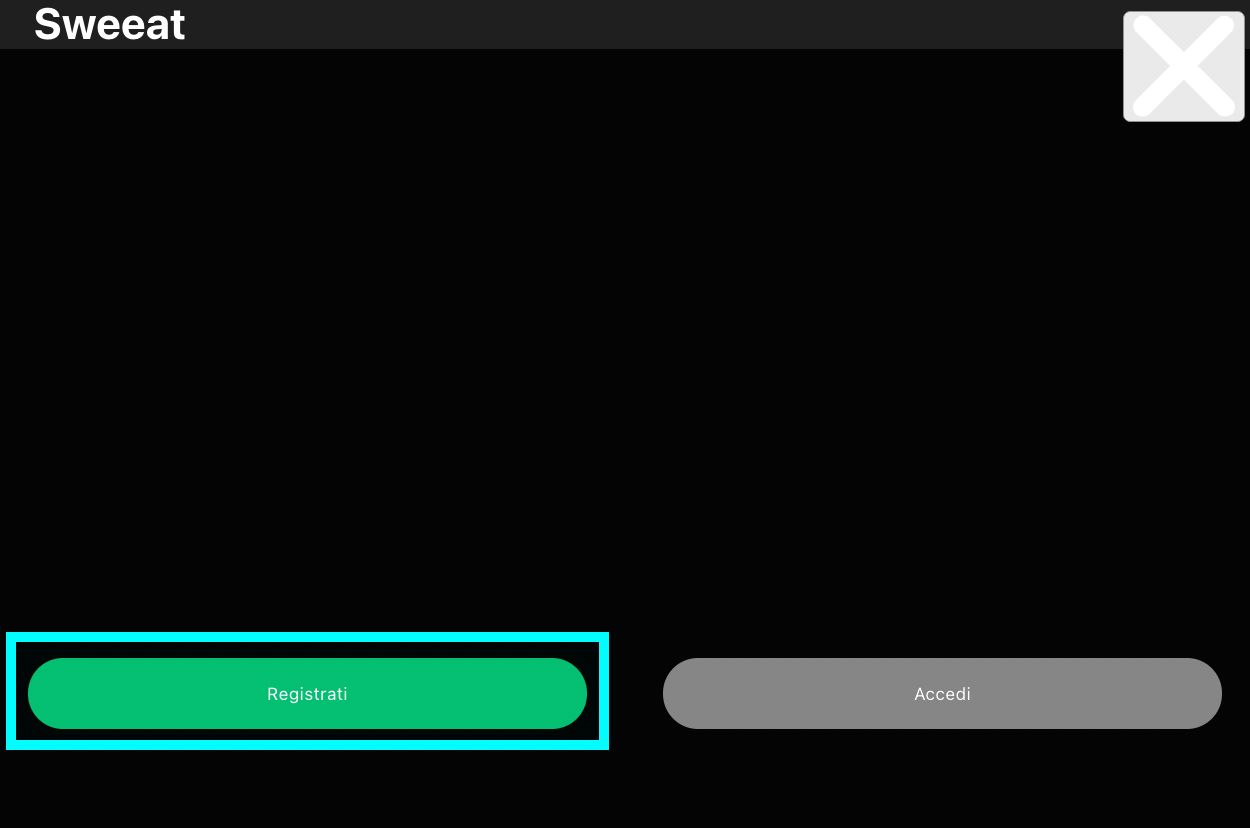
\includegraphics[scale=0.2]{./images/Registrazione/RegMobile.png} 
\caption{Bottone di registrazione versione mobile}
\end{figure}

Una volta cliccato sul bottone, l’utente verrà reindirizzato in una nuova pagina contenente un modulo, nel quale dovrà inserire i dati per la registrazione.

\begin{figure}[H]
\centering
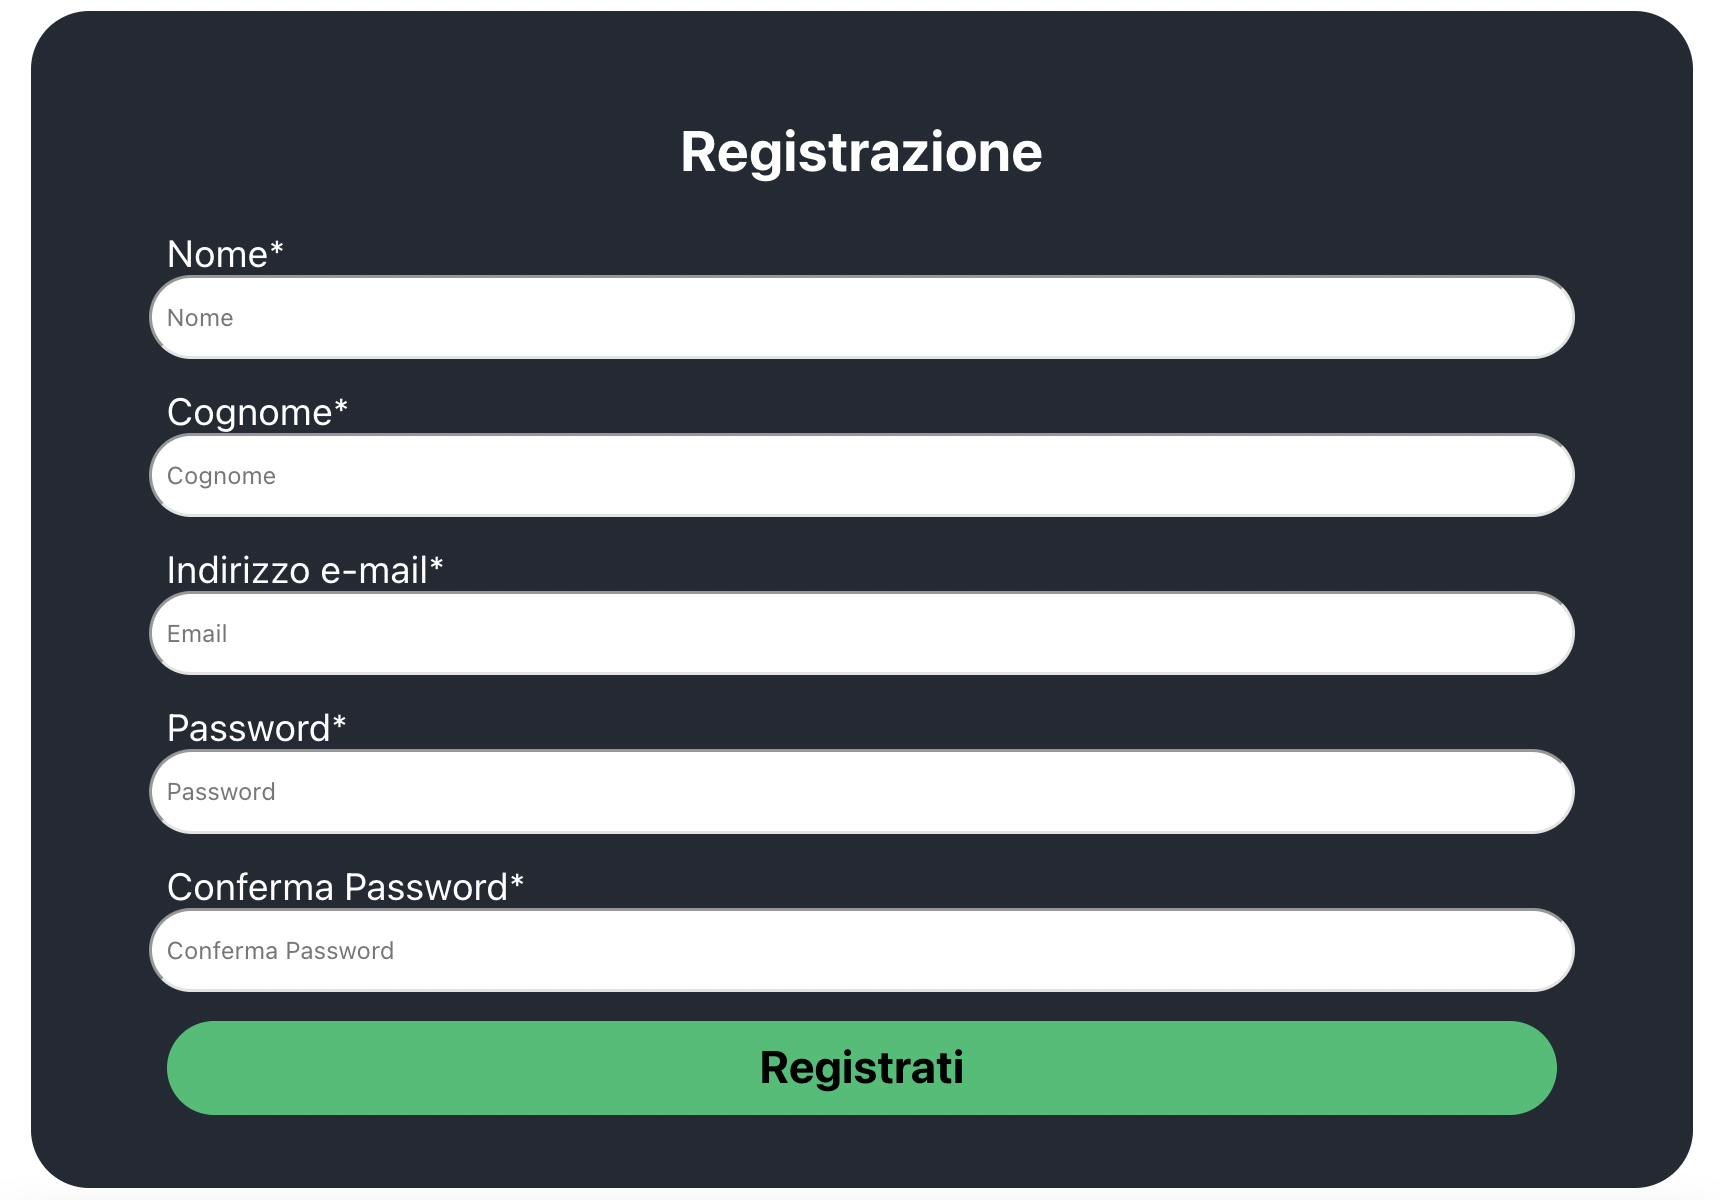
\includegraphics[scale=0.3]{./images/Registrazione/FormRegistrazione.png} 
\caption{Modulo di registrazione a Sweeat}
\end{figure}

I dati(*) da inserire in fase di registrazione sono:

\begin{itemize}
\item \textbf{Nome},
\item \textbf{Cognome},
\item \textbf{Indirizzo e-mail}, 
\item \textbf{Password}, (che dovrà essere lunga almeno 8 caratteri e contenere almeno una lettera maiuscola, una minuscola, un numero ed un simbolo tra i seguenti: @ \$ ! \% * ? \&). 
\end{itemize}

(*) tutti i dati richiesti sono obbligatori. \\

L’indirizzo e-mail e la password serviranno per accedere all'account personale nella piattaforma.

Dopo aver inserito tutti i dati richiesti, per effettuare la registrazione sarà necessario cliccare sul bottone “\textbf{Registrati}”.

Una volta fatto ciò, comparirà il seguente messaggio di benvenuto: 

\begin{figure}[H]
\centering
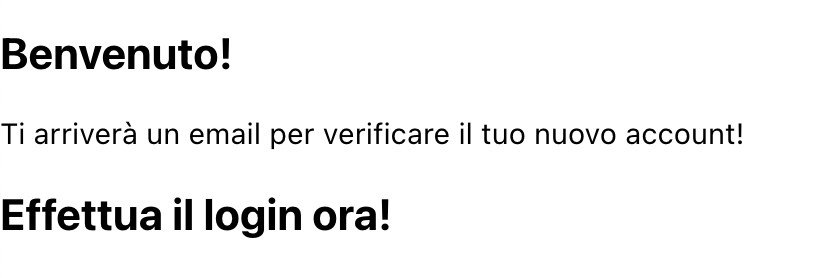
\includegraphics[scale=0.5]{./images/Registrazione/Welcome.png} 
\caption{Messaggio di Benvenuto su Sweeat}
\end{figure}

e sarà necessario confermare la propria identità cliccando sul link che verrà inviato all’indirizzo e-mail inserito in fase di registrazione.

\begin{figure}[H]
\centering

\includegraphics[scale=0.5]{./images/Registrazione/emailReg.png} 
\caption{E-mail di conferma dell'identità}
\end{figure}

Una volta confermato l’account, comparirà il seguente messaggio di conferma:

\begin{figure}[H]
\centering
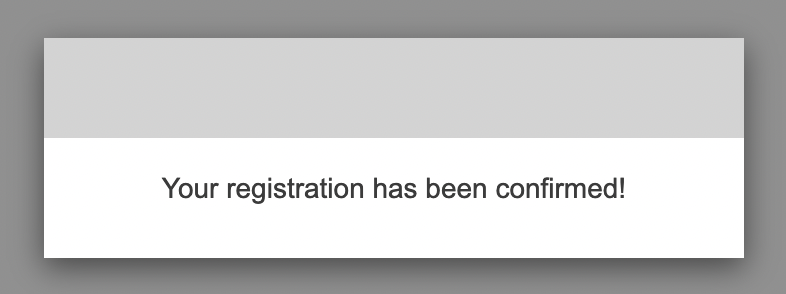
\includegraphics[scale=0.5]{./images/Registrazione/Conferma.png} 
\caption{Conferma di avvenuta registrazione su Sweeat}
\end{figure}

e sarà possibile accedere alla propria \textbf{Area Personale}.

\subsection{Inserimento Dati Errati}

Nel caso in cui l'utente voglia procedere con la registrazione lasciando uno o più campi vuoti, la registrazione non andrà a buon fine ed il sistema mostrerà i seguenti errori:

\begin{figure}[H]
\centering
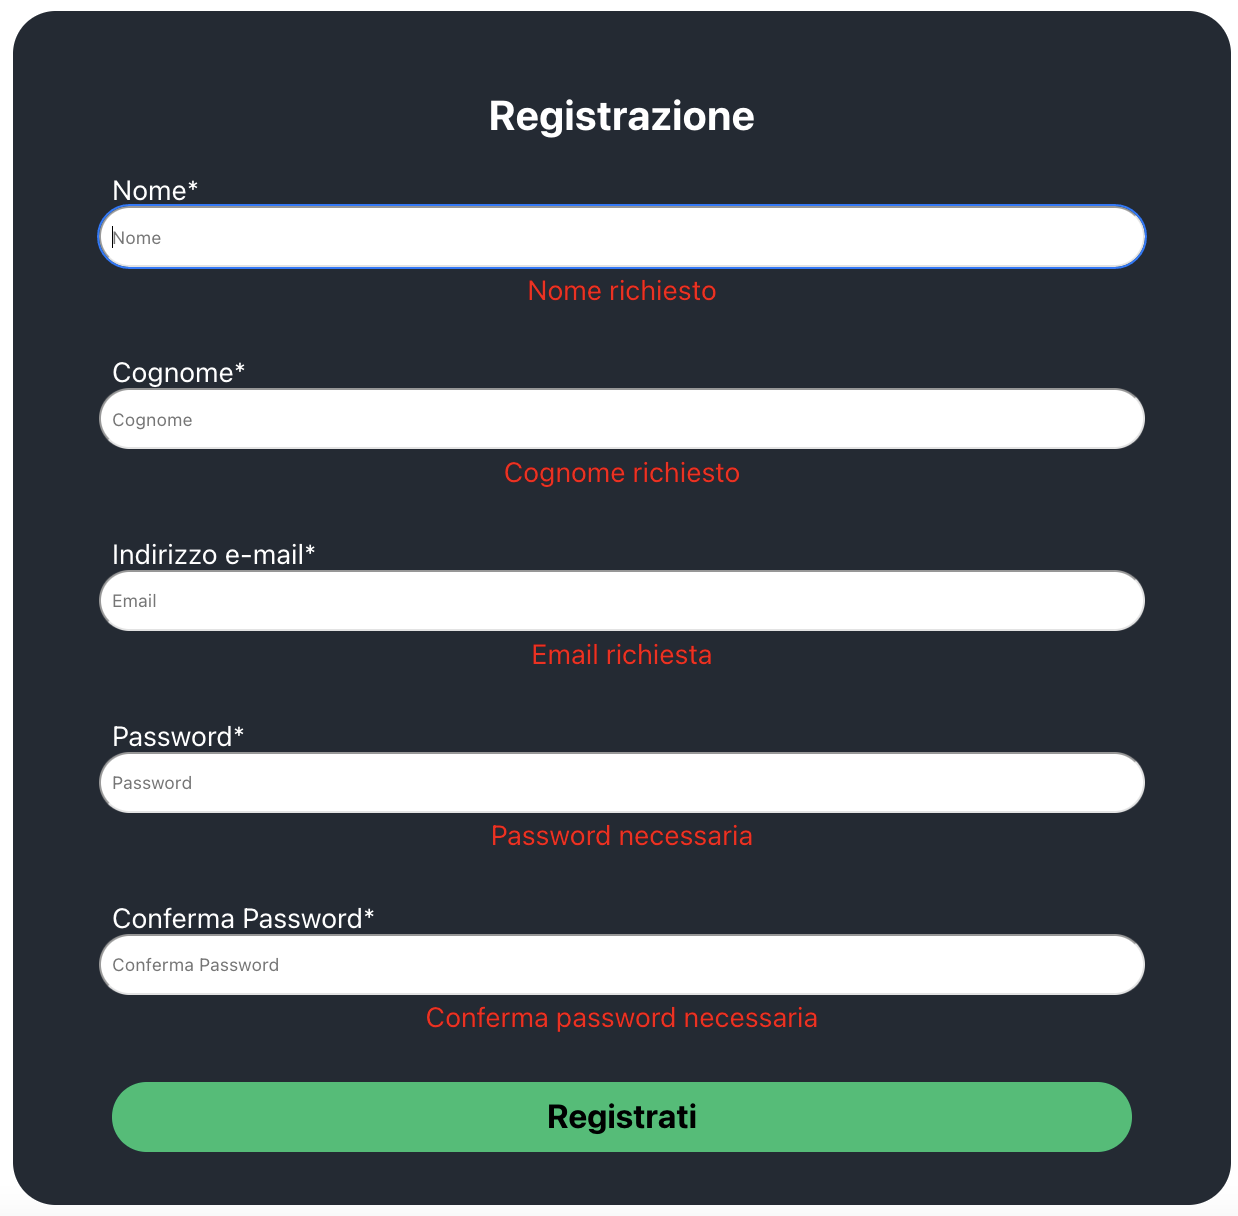
\includegraphics[scale=0.4]{./images/Registrazione/DatiErrati.png} 
\caption{Errori nell'inserimento dei dati in fase di registrazione}
\end{figure}

Affinché la registrazione vada a buon fine, è necessario compilare correttamente tutti i campi. 

		
		\section{Login}
		% Login

È possibile accedere al modulo di accesso tramite il seguente link:

\begin{center}
\textsl{ \href{https://dev.d1ay0almkohcfw.amplifyapp.com/login}{\textbf{https://dev.d1ay0almkohcfw.amplifyapp.com/login} }}
\end{center}

Accedere alla propria Area Personale (\S{4}) è molto semplice; dopo aver cliccato sul bottone “\textbf{Accedi}” nella barra di navigazione (in alto a destra nella versione Desktop e dal menù a tendina nella versione mobile), l’utente verrà reindirizzato in una nuova pagina.

\begin{figure}[H]
\centering

\includegraphics[scale=0.15]{./images/Login/LoginDesktop.png} 
\caption{Bottone di accesso versione desktop}
\end{figure}

\begin{figure}[H]
\centering
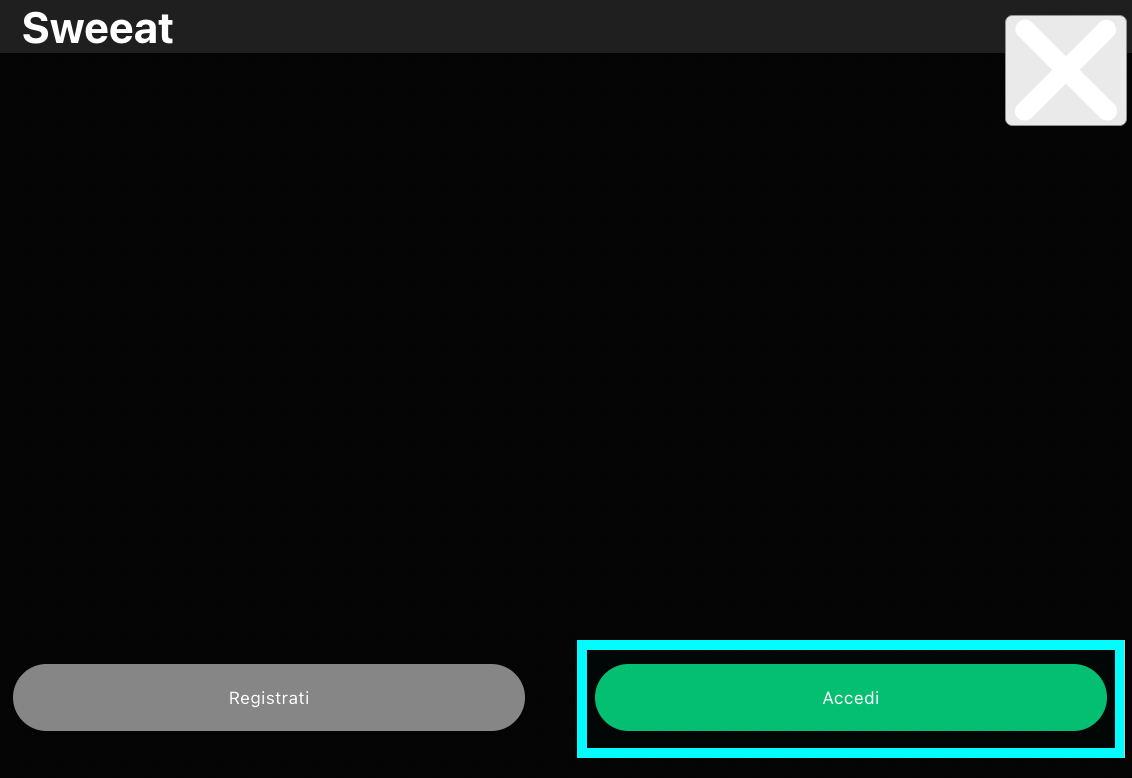
\includegraphics[scale=0.2]{./images/Login/LoginMobile.png} 
\caption{Bottone di accesso versione mobile}
\end{figure}

In questa nuova pagina comparirà un modello da compilare, nel quale l’utente dovrà inserire i seguenti dati personali:

\begin{enumerate}
\item \textbf{Indirizzo e-mail},
\item \textbf{Password}.
\end{enumerate}

\begin{figure}[H]
\centering
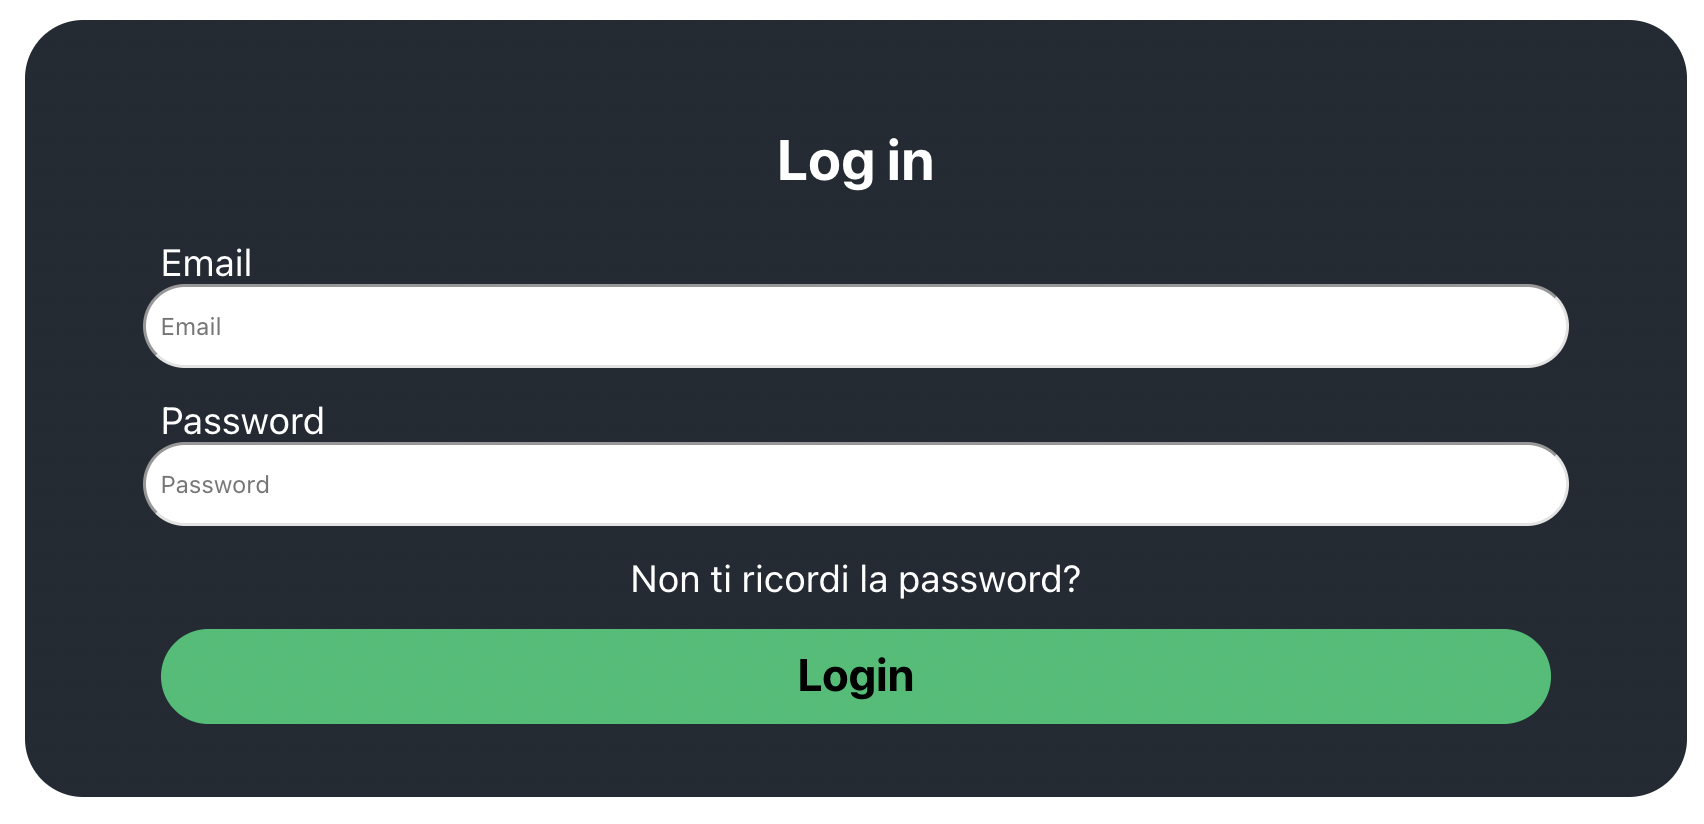
\includegraphics[scale=0.3]{./images/Login/FormLogin.png} 
\caption{Modulo di accesso da compilare per accedere a Sweeat}
\end{figure}

Entrambi i campi sono obbligatori ed i dati sono quelli inseriti in fase di registrazione (\S{4}). 

Una volta inseriti i dati, per accedere all’area personale sarà sufficiente cliccare sul bottone “\textbf{Login}”.

Dopo aver effettuato l’accesso, sarà possibile navigare nella propria \textbf{Area Personale}.

\subsection{Inserimento credenziali errate}

Nel caso in cui l'utente non inserisca le credenziali di accesso nel form di login, compariranno i seguenti errori: 

\begin{figure}[H]
\centering
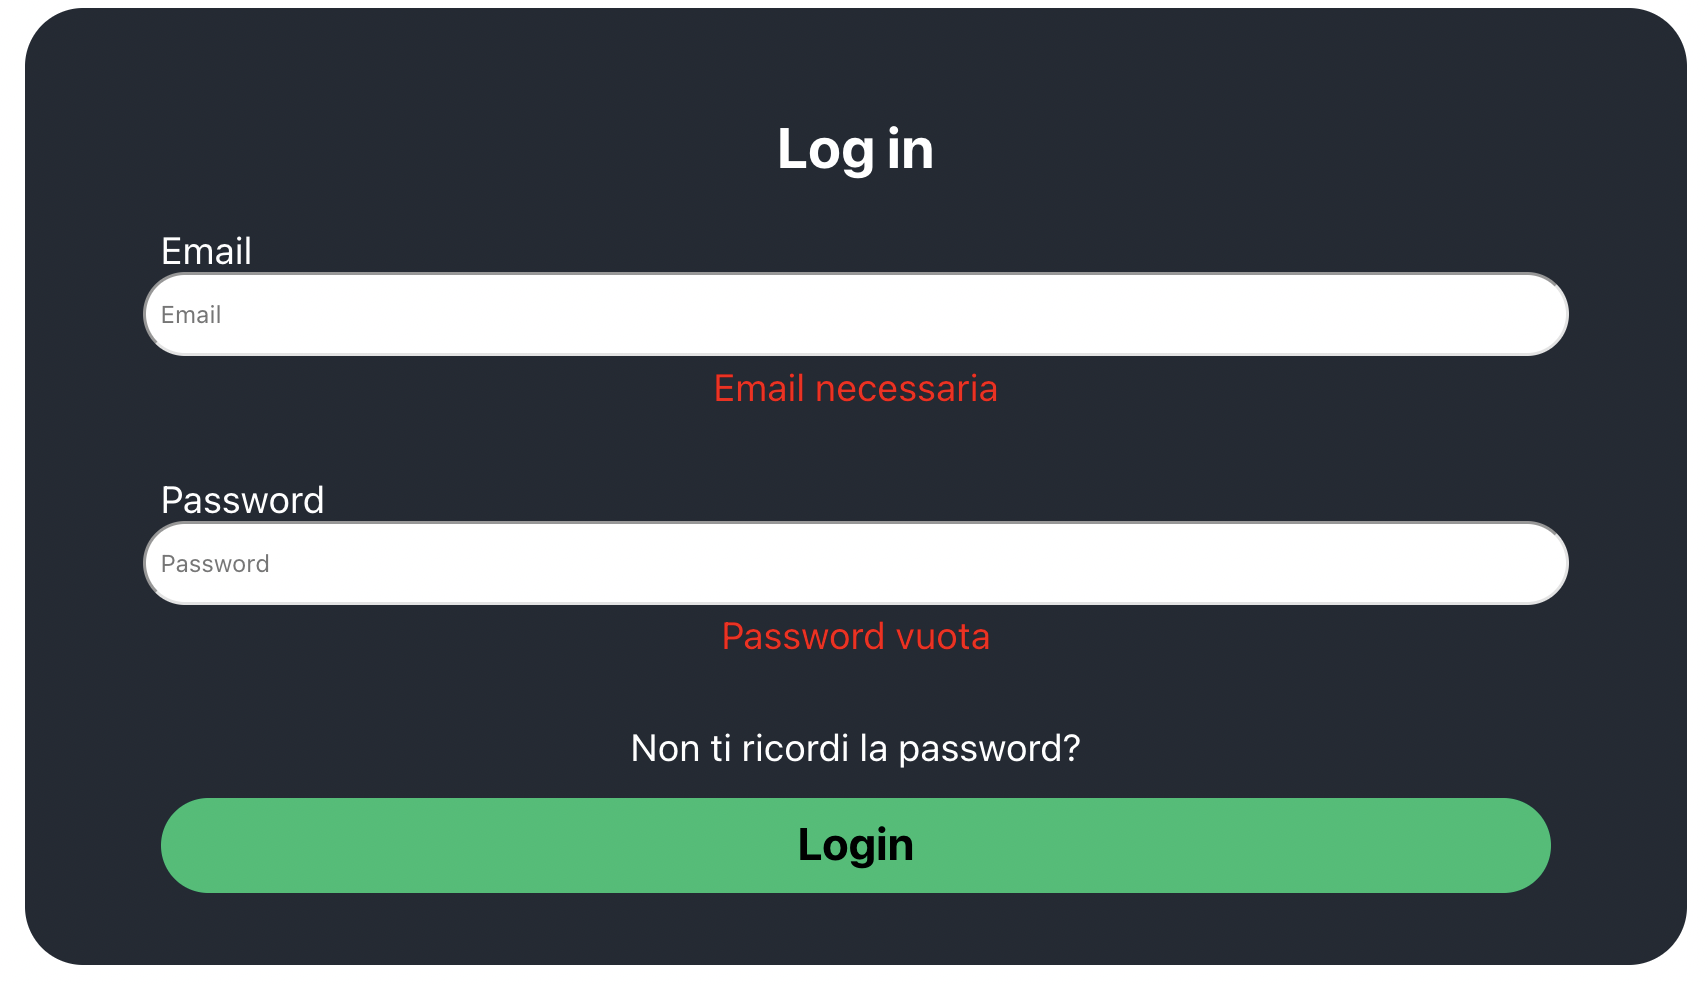
\includegraphics[scale=0.3]{./images/Login/ErroreCampi.png} 
\caption{Credenziali per il login non inserite}
\end{figure}

Per procedere, è necessario inserire le credenziali di accesso inserite in fase di registrazione (\S{4}), oppure procedere con il recupero password (\S{6}). 

Analogamente, nel caso in cui l'utente non inserisca delle credenziali corrette, all'utente verrà mostrato il seguente errore:

\begin{figure}[H]
\centering
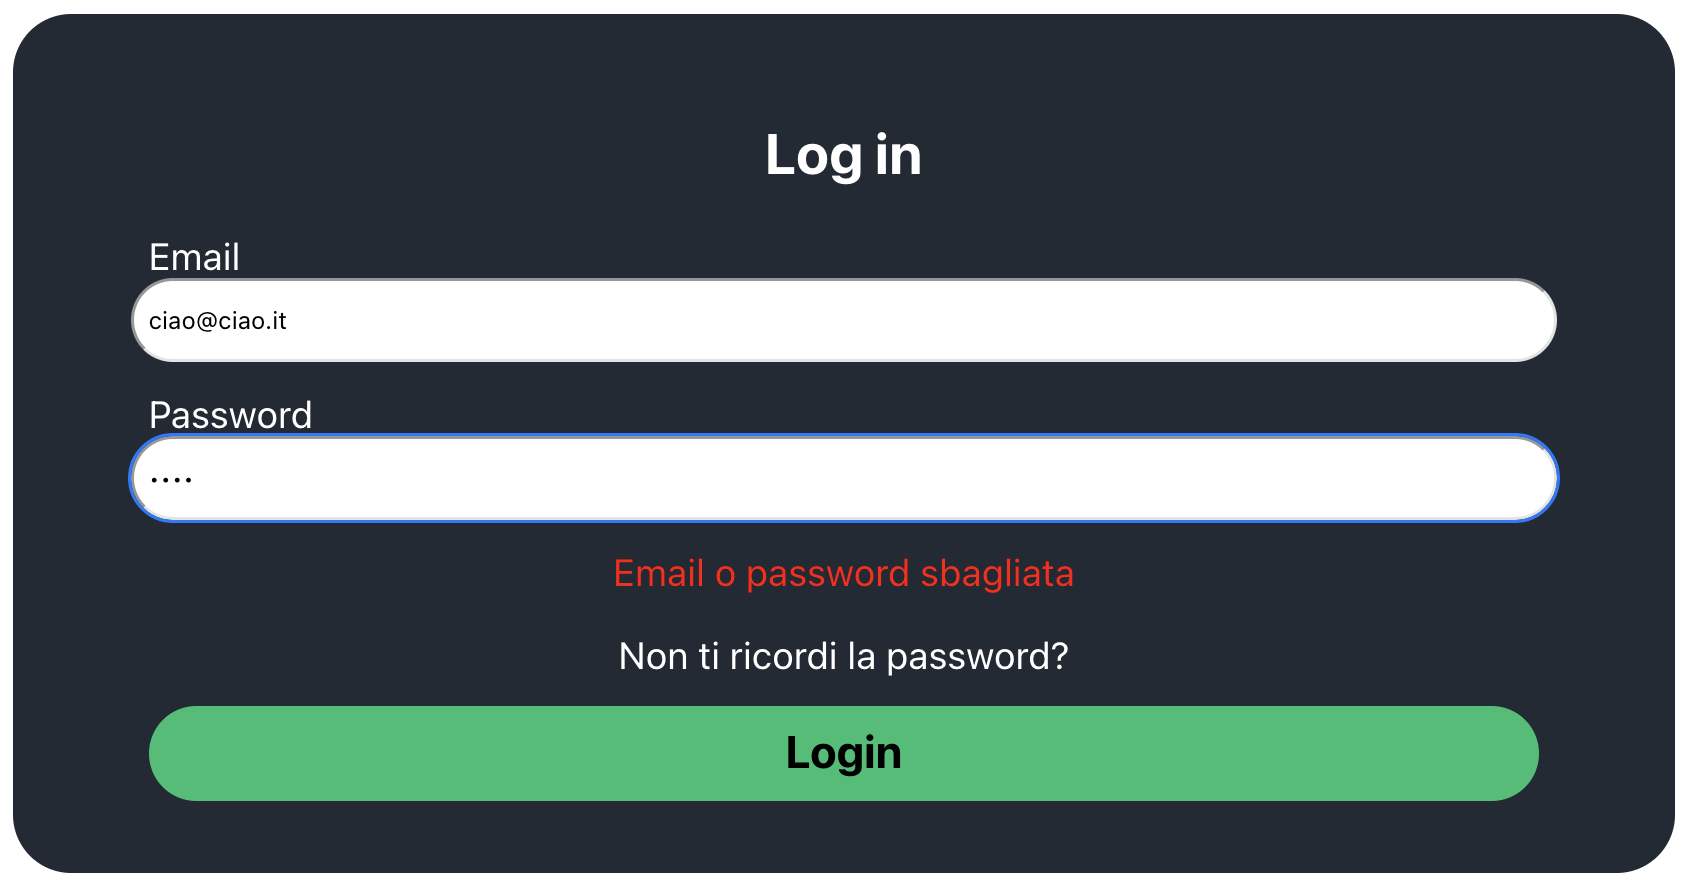
\includegraphics[scale=0.3]{./images/Login/AccessoNegato.png} 
\caption{Errore nell'inserimento delle credenziali per effettuare l'accesso}
\end{figure}

\subsection{Logout}

Un utente che ha effettuato l'accesso nella piattaforma, può “sloggarsi” cliccando sulla voce “\textbf{Log out}” presente nella barra di navigazione in ogni pagina del sito.

\begin{figure}[H]
\centering

\includegraphics[scale=0.15]{./images/Login/Logout.png} 
\caption{Logout da Sweeat}
\end{figure}

Se l'utente non ricorda più la password di accesso, potrà recuperarla tramite l'operazione di recupero password (\S{6}).
		
		\section{Recupero Password}
		% Recupero Password

Nel caso in cui l'utente avesse smarrito o si fosse dimenticato la password di accesso inserita in fase di registrazione (\S{4}), è possibile cambiarla inserendone una nuova.

\begin{center}
\textsl{ \href{https://dev.d1ay0almkohcfw.amplifyapp.com/passwordDimenticata}{\textbf{https://dev.d1ay0almkohcfw.amplifyapp.com/passwordDimenticata} }}
\end{center}

Per fare ciò, anziché compilare il modulo di Login (\S{5}), l'utente dovrà cliccare sulla voce “Non ti ricordi la password?”

\begin{figure}[H]
\centering
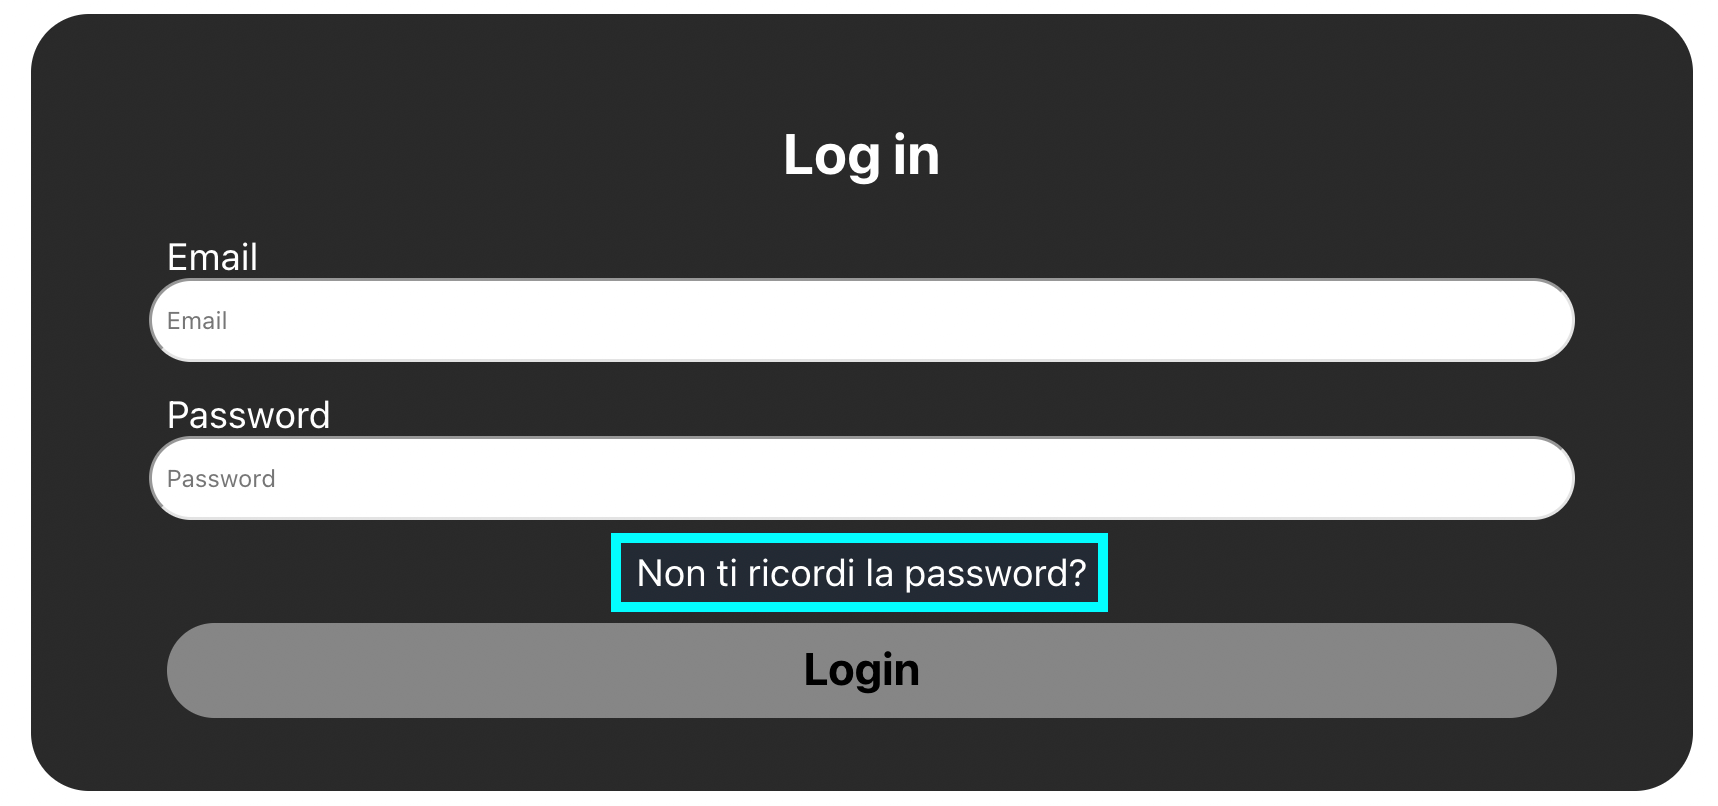
\includegraphics[scale=0.2]{./images/RecuperoPassword/Login.png} 
\caption{Bottone per il recupero password}
\end{figure}

ed inserire l'indirizzo e-mail tramite il quale si vuole verificare l'identità per cambiare la password di accesso.

\begin{figure}[H]
\centering
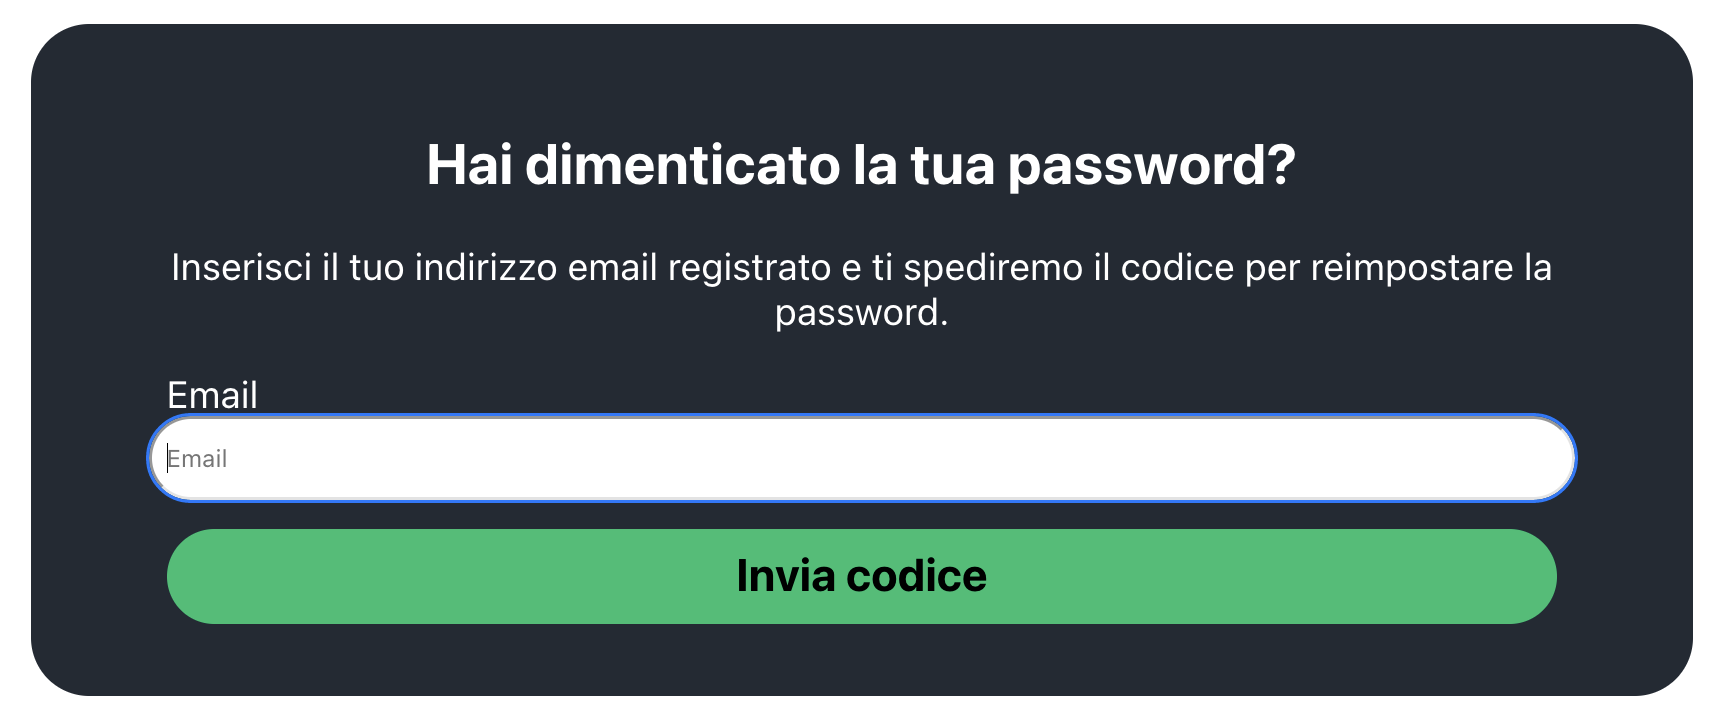
\includegraphics[scale=0.3]{./images/RecuperoPassword/FormRecuperoPwd.png} 
\caption{Form per il recupero password}
\end{figure}

Una volta inserito l'indirizzo e-mail, sarà possibile recuperare la password compilando il form (ossia inserendo l'indirizzo e-mail inserito in fase di registrazione (\S{4})), quindi clicca su “Invia codice”. Riceverai via e-mail un codice numerico di sei cifre, che ti servirà per il prossimo passaggio.

\begin{figure}[H]
\centering
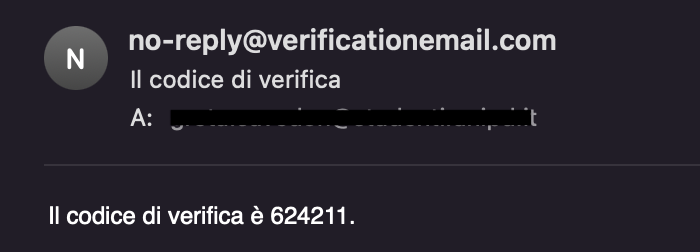
\includegraphics[scale=0.45]{./images/RecuperoPassword/emailRecupero.png} 
\caption{Codice numerico per il recupero password}
\end{figure}

Ora dovrai inserire una nuova password nel form, oltre al codice che avrai ricevuto via e-mail (l'indirizzo e-mail verrà inserito automaticamente).

\begin{figure}[H]
\centering
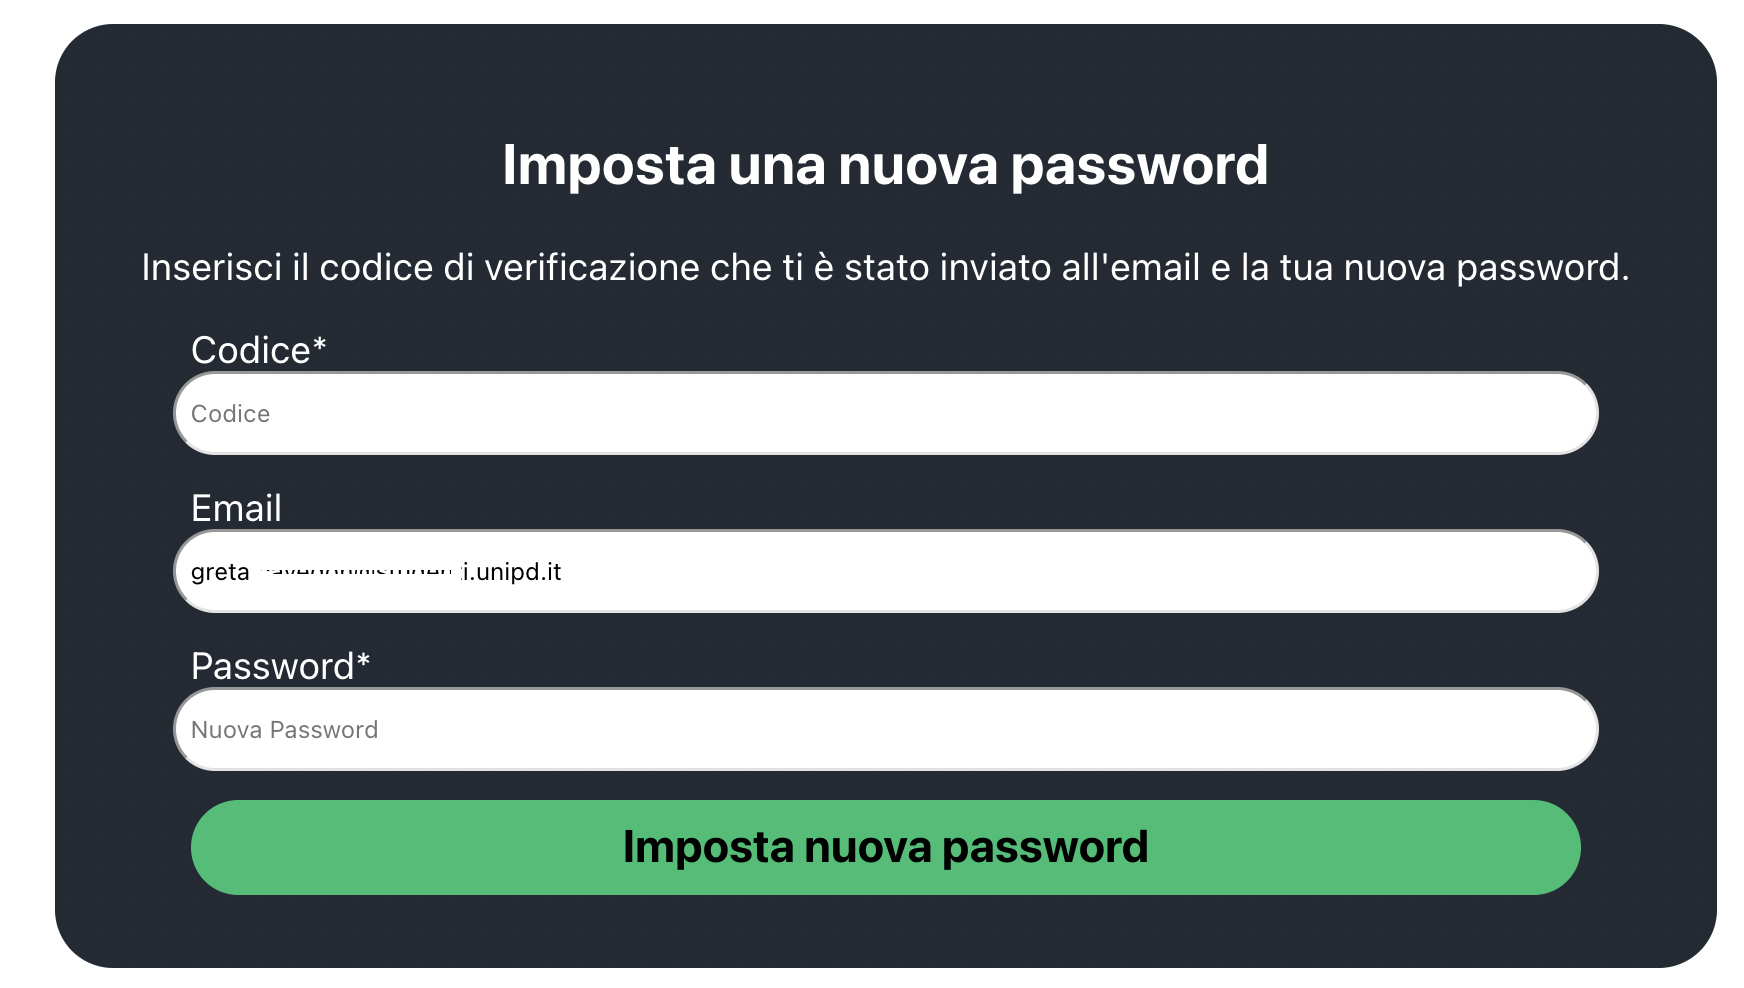
\includegraphics[scale=0.3]{./images/RecuperoPassword/FormNuovaPsw.png} 
\caption{Bottone di registrazione versione desktop}
\end{figure}

Successivamente dovrai cliccare su “\textbf{Imposta nuova password}” e, nel caso il cambio sia andato a buon fine, visualizzare il seguente messaggio:

\begin{figure}[H]
\centering
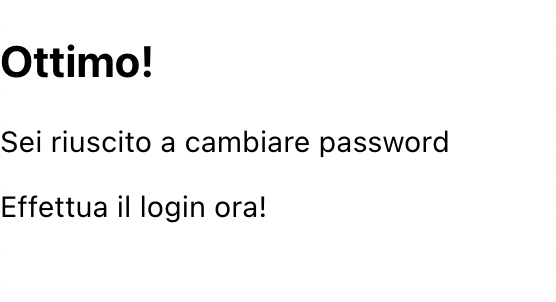
\includegraphics[scale=0.5]{./images/RecuperoPassword/cambioRiusciuto.png} 
\caption{Bottone di registrazione versione desktop}
\end{figure}

Effettua ora il login (\S{5}) per accedere alla tua Area Personale (\S{7}).

		
		\section{Area Personale}
		% Area Personale
L’utente registrato e che ha effettuato l’accesso nella piattaforma web, avrà un’area personale nella quale:

\begin{itemize}
\item Visualizzare i propri dati personali (\S{7.1}),
\item Modificare la password di accesso al sistema (\S{7.2}),
\item Suggerire un profilo Instagram che potrebbe essere utile alla piattaforma (\S{7.3}),
\item Visualizzare e gestire la propria lista dei preferiti (\S{7.4}).
\end{itemize}

È possibile scegliere una di queste operazioni dalla sezione “Area Personale” (sia per la versione desktop che mobile), la quale aprirà una nuova finestra a seconda della funzionalità scelta.

\subsection{Visualizza dati personali}

L’utente registrato e che ha effettuato l’accesso alla piattaforma web può visualizzare i propri dati personali inseriti in fase di registrazione.

I dati personali che un utente può visualizzare nella sua Area Personale (alla sezione “Dati Personali”) sono:

\begin{itemize}
\item Nome,
\item Cognome,
\item Indirizzo e-mail.
\end{itemize}

\begin{figure}[H]
\centering
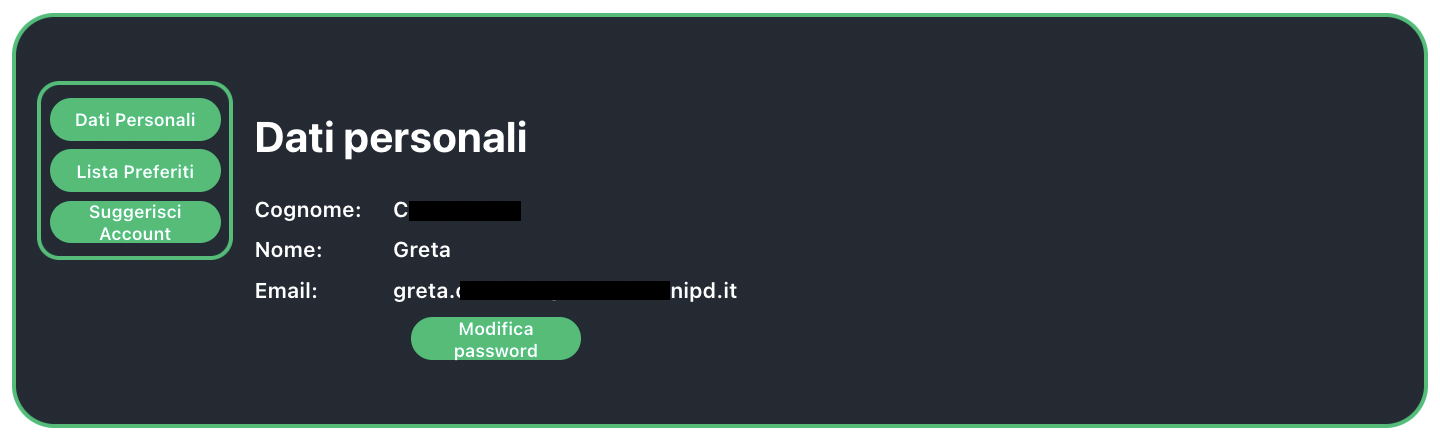
\includegraphics[scale=0.4]{./images/AreaPersonale/DatiPersonali.png} 
\caption{Suggerisci profilo}
\end{figure}

Da questa schermata l’utente può anche modificare la propria password (come indicato nel paragrafo che segue).

\subsection{Modifica password}

L’utente registrato e che ha effettuato il proprio accesso al sistema ha la possibilità di modificare la propria password di accesso.

Per fare ciò, dalla sezione denominata “Dati Personali”, l'utente dovrà cliccare sul bottone “\textbf{Modifica Password}” ed inserire una nuova password, avendo cura di inserire almeno: 8 caratteri e che contengono almeno una lettera maiuscola, una minuscola, un numero ed un simbolo tra i seguenti: @ \$ ! \% * ? \&{}.

\begin{figure}[H]
\centering
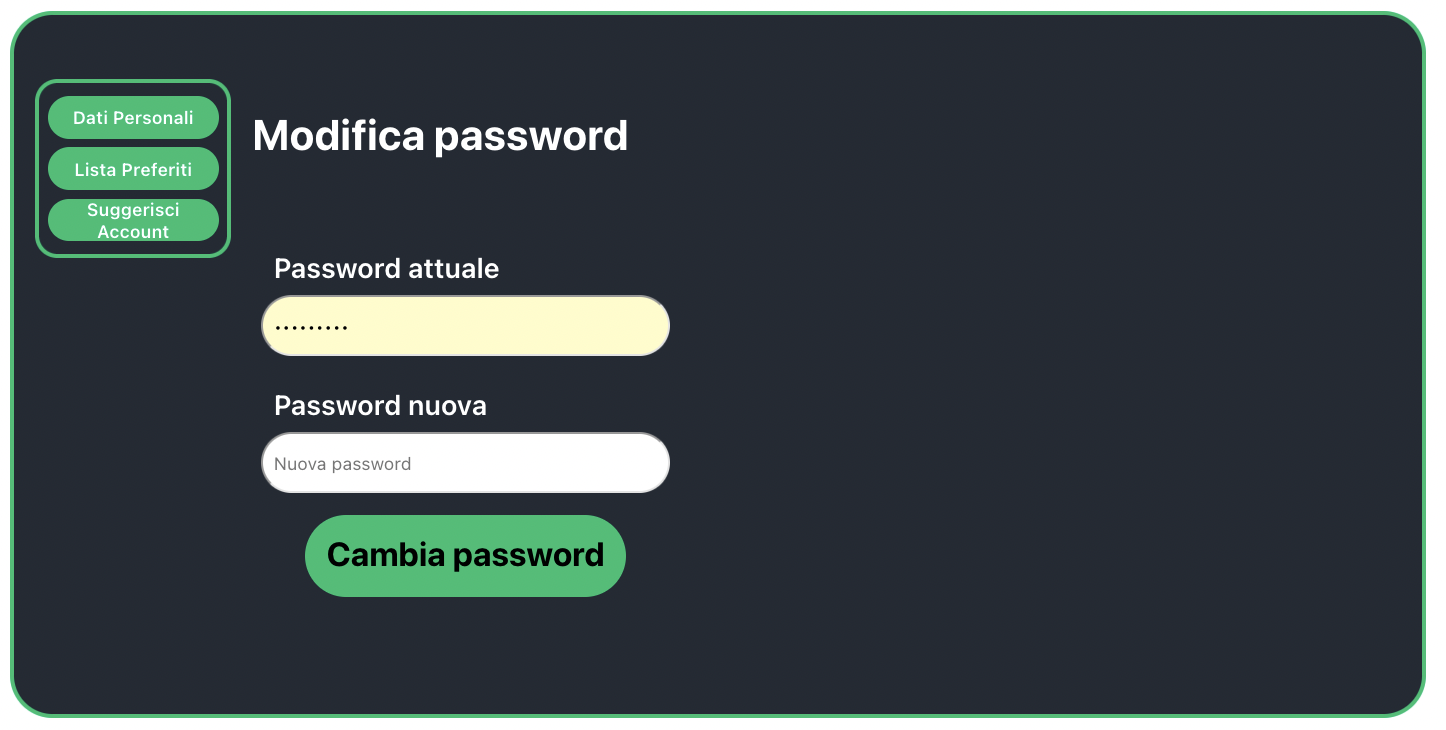
\includegraphics[scale=0.4]{./images/AreaPersonale/CambiaPassword.png} 
\caption{Suggerisci profilo}
\end{figure}

\subsection{Suggerisci un profilo}

Un utente registrato alla piattaforma e che ha effettuato l’accesso ha l’opportunità di suggerire un profilo Instagram al sistema.

Per fare ciò, dalla pagina “Area Personale” un utente può cliccare sulla voce “Suggerisci un profilo”, dalla quale comparirà una casella di testo:

\begin{figure}[H]
\centering
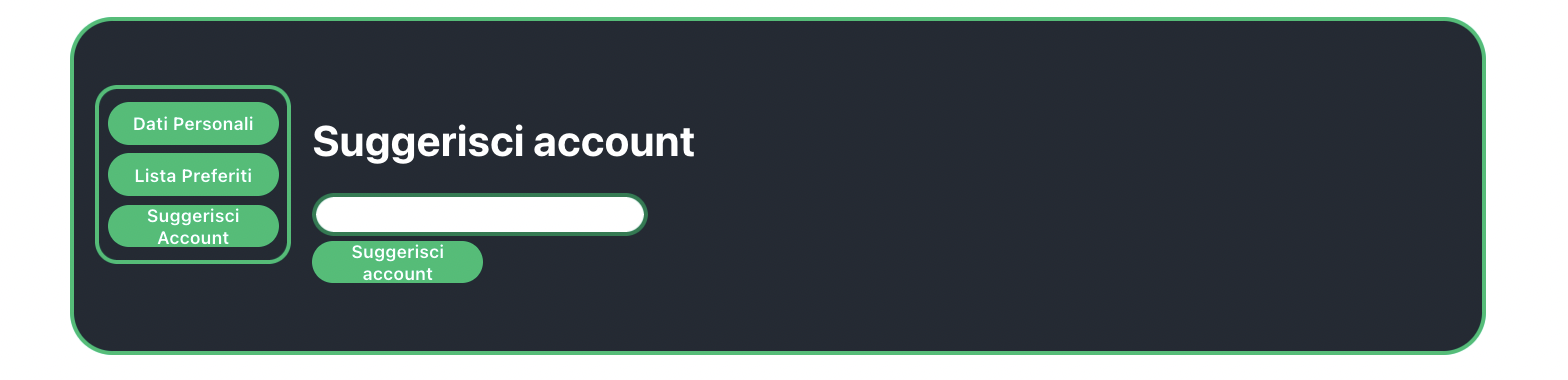
\includegraphics[scale=0.4]{./images/AreaPersonale/SuggerisciAccount.png} 
\caption{Suggerisci profilo}
\end{figure}

Al suo interno, l’utente potrà inserire il nome utente del profilo Instagram da suggerire alla piattaforma. Questa funzionalità non è ancora stata implementata.

\subsection{Lista dei preferiti}

Un utente registrato e che ha effettuato l’accesso alla piattaforma ha l’opportunità rimuovere locali dalla propria lista dei preferiti direttamente dall'Area Personale. \\

Dalla sezione “Area Personale”, l’utente autenticato può cliccare su “Lista dei preferiti” dove visualizzerà o una lista vuota, nel caso nella lista non ci sia alcun locale preferito, o una lista con dei locali presenti a sistema.

\begin{figure}[H]
\centering
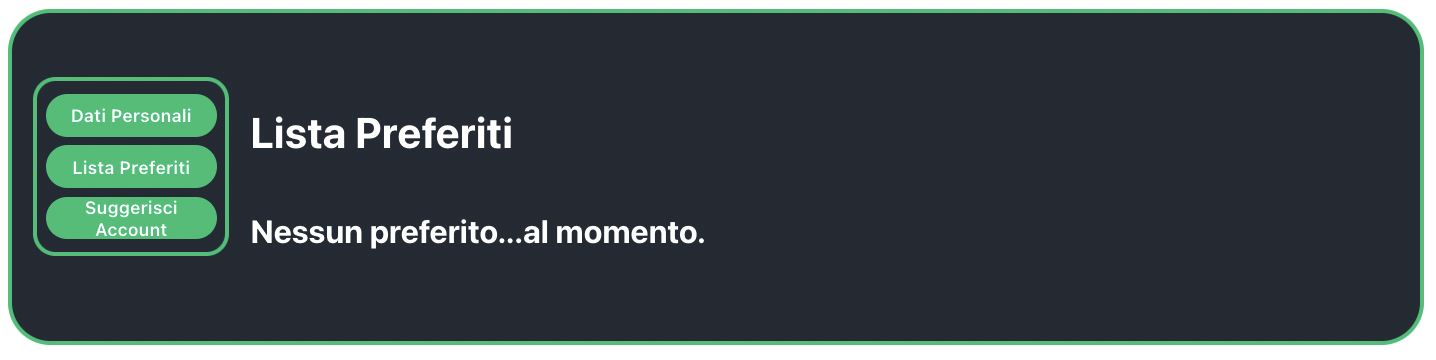
\includegraphics[scale=0.4]{./images/AreaPersonale/ListaPreferiti.png} 
\caption{Lista dei locali preferiti}
\end{figure}

L’utente può rimuovere un locale dalla lista dei preferiti semplicemente cliccando sull’icona del cestino.

In questo modo, il locale verrà rimosso dalla lista e sarà necessario cercarlo (tramite la ricerca \S{8.1}) per aggiungerlo nuovamente. Questo meccanismo di aggiungere e rimuovere un locale dalla lista dei preferiti è una funzionalità che non è ancora stata implementata.


		\section{Homepage}
		% Pagina iniziale
Dalla pagina iniziale del sito è possibile:

\begin{itemize}
\item Effettuare una ricerca (\S{8.1}),
\item Visualizzare una classifica con i migliori locali presenti su sito (\S{8.2}).  
\end{itemize}

\begin{figure}[H]
\centering
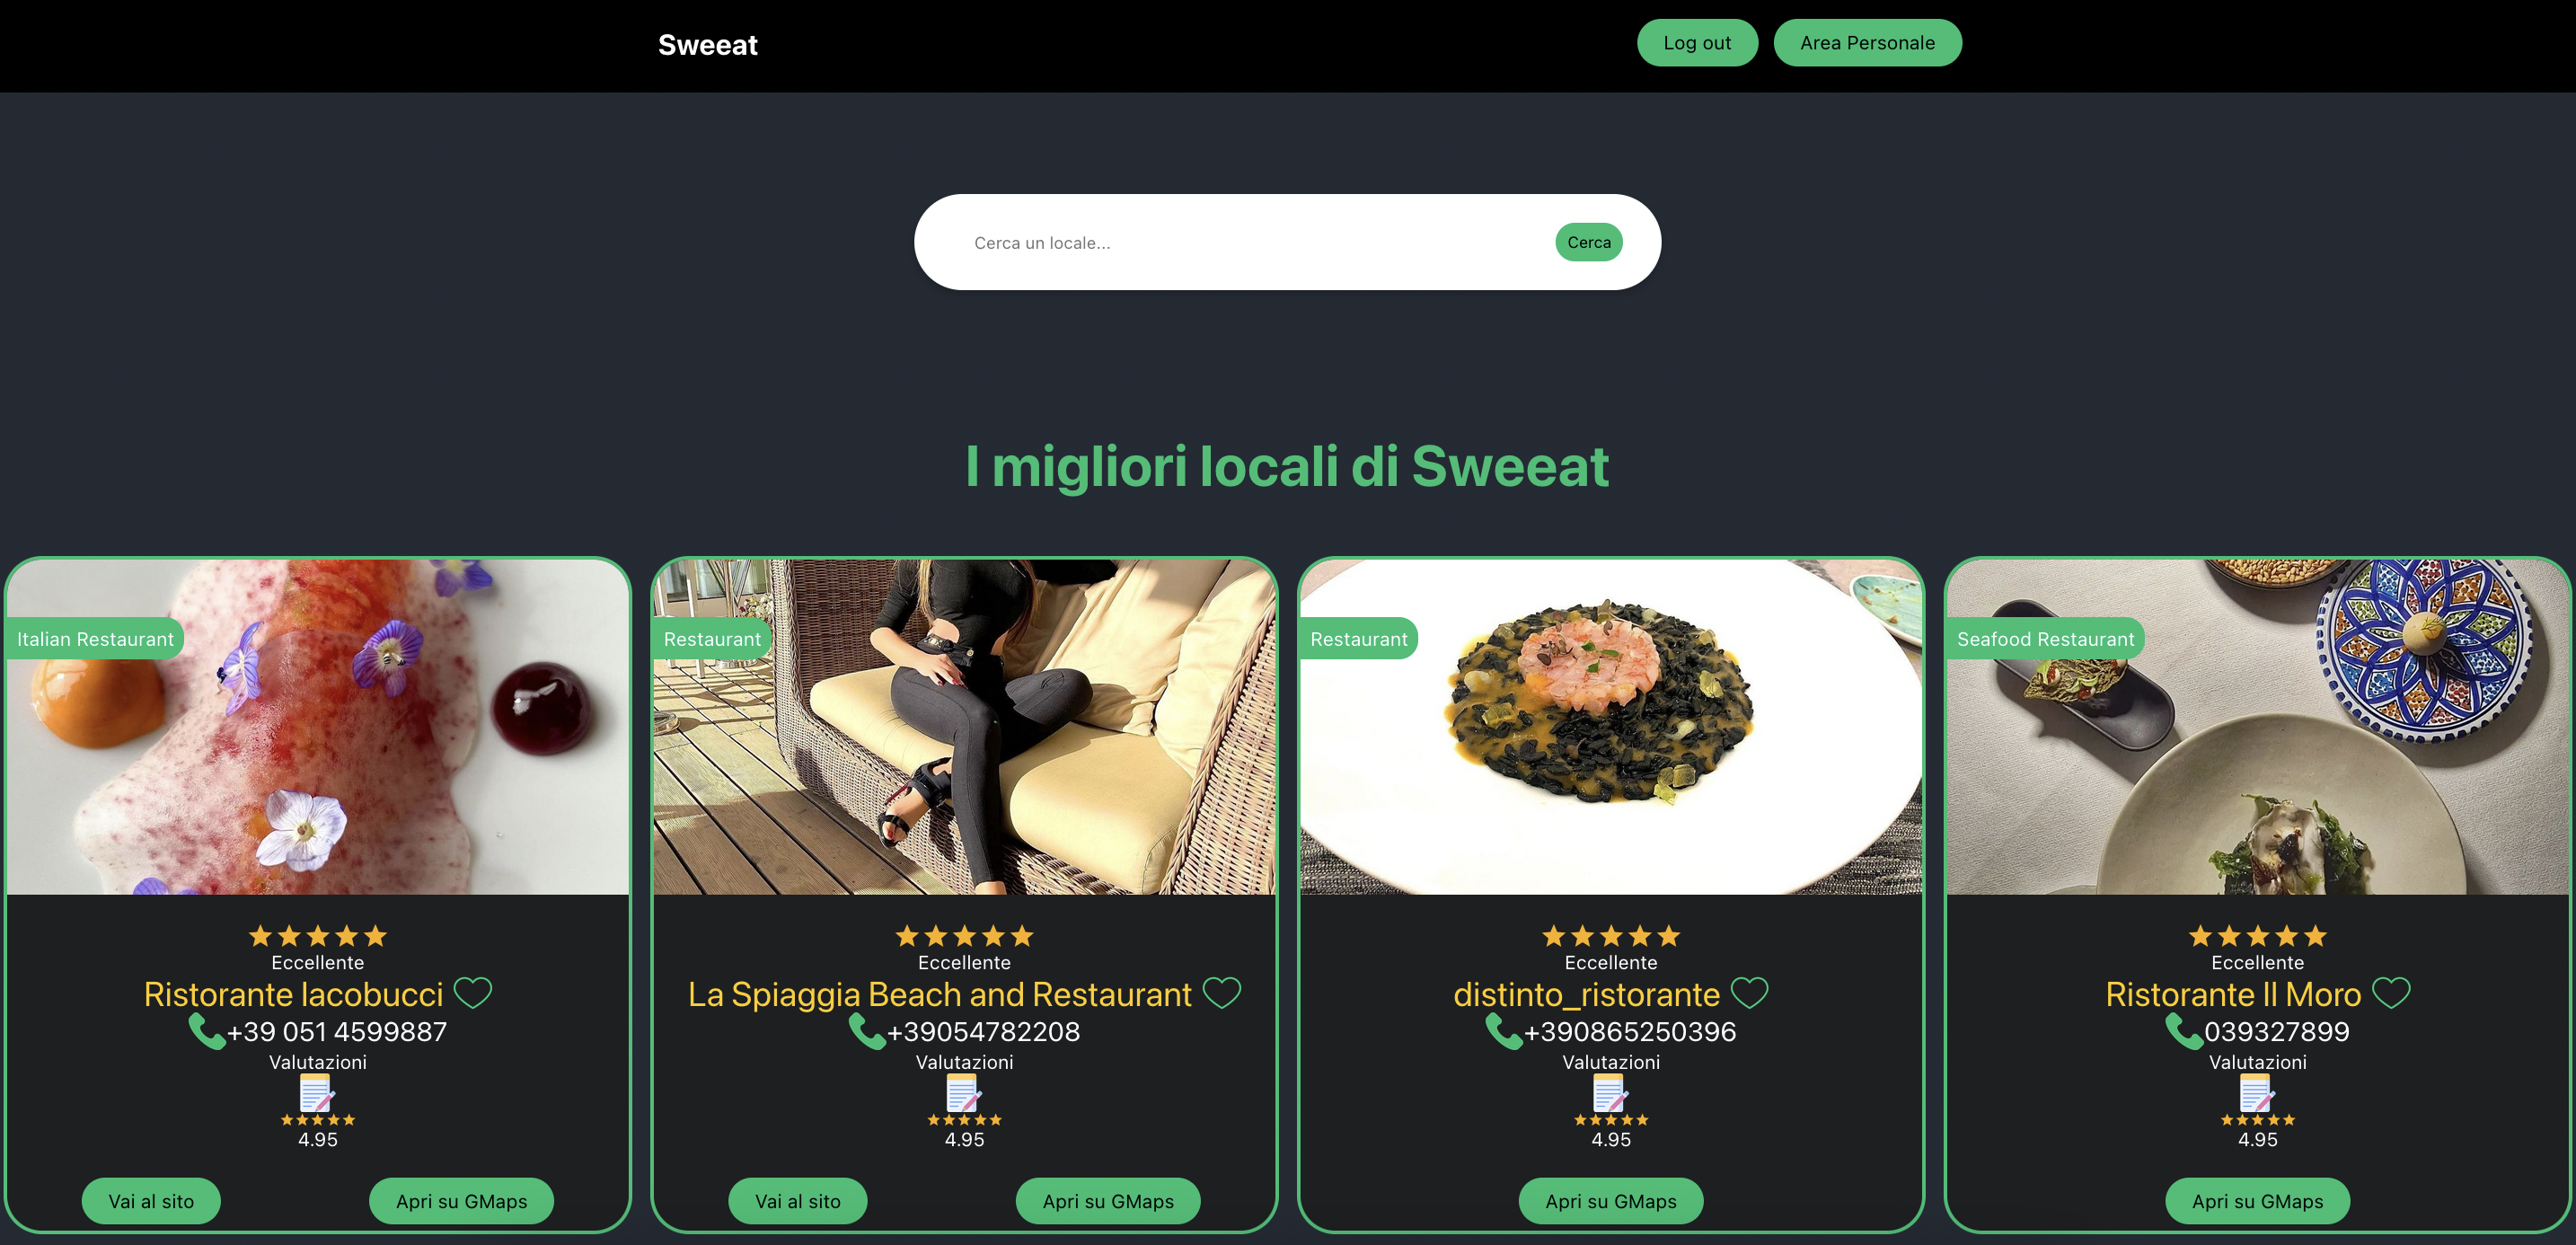
\includegraphics[scale=0.3]{./images/Homepage/Homepage.png} 
\caption{Homepage}
\end{figure}

\subsection{Ricerca}

Per effettuare una ricerca è necessario inserire il \textbf{nome del locale} cercato.

\begin{figure}[H]
\centering
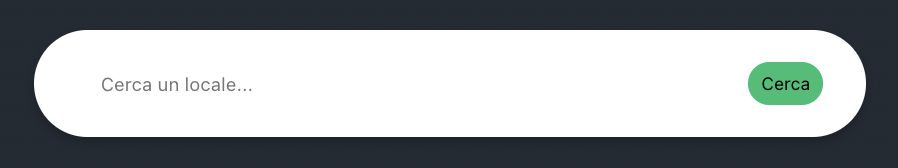
\includegraphics[scale=0.45]{./images/Homepage/Ricerca.png} 
\caption{Barra di ricerca nella Homepage}
\end{figure}

Quindi, va inserito il nome del locale da cercare e, per avviare la ricerca, è necessario cliccare su “\textbf{Cerca}”.

\begin{figure}[H]
\centering
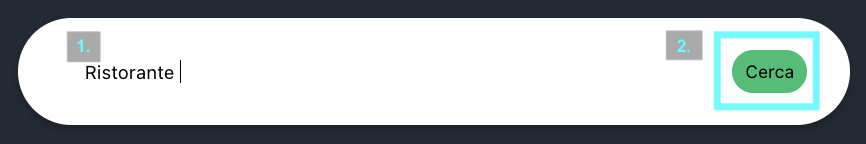
\includegraphics[scale=0.5]{./images/Homepage/Ricerca2.png} 
\caption{Inserimento dati ed avvio ricerca in Homepage}
\end{figure}

Una volta fatto ciò, verrà avviata la ricerca e l’utente verrà reindirizzato nella pagina dei risultati (\S{9}), la quale conterrà il risultato della ricerca (ossia, il locale cercato, dei locali alternativi o nessun locale).

\subsection{Visualizzare i migliori locali presenti su Sweeat}

Dalla pagina iniziale, oltre ad effettuare una ricerca, è possibile visualizzare i quattro migliori locali presenti nella piattaforma ed interagire con essi.

La sezione dedicata ai quattro migliori locali della piattaforma si trova sotto alla sezione contenente la barra di ricerca (sotto alla voce “I migliori locali di Sweeat”).

\begin{figure}[H]
\centering
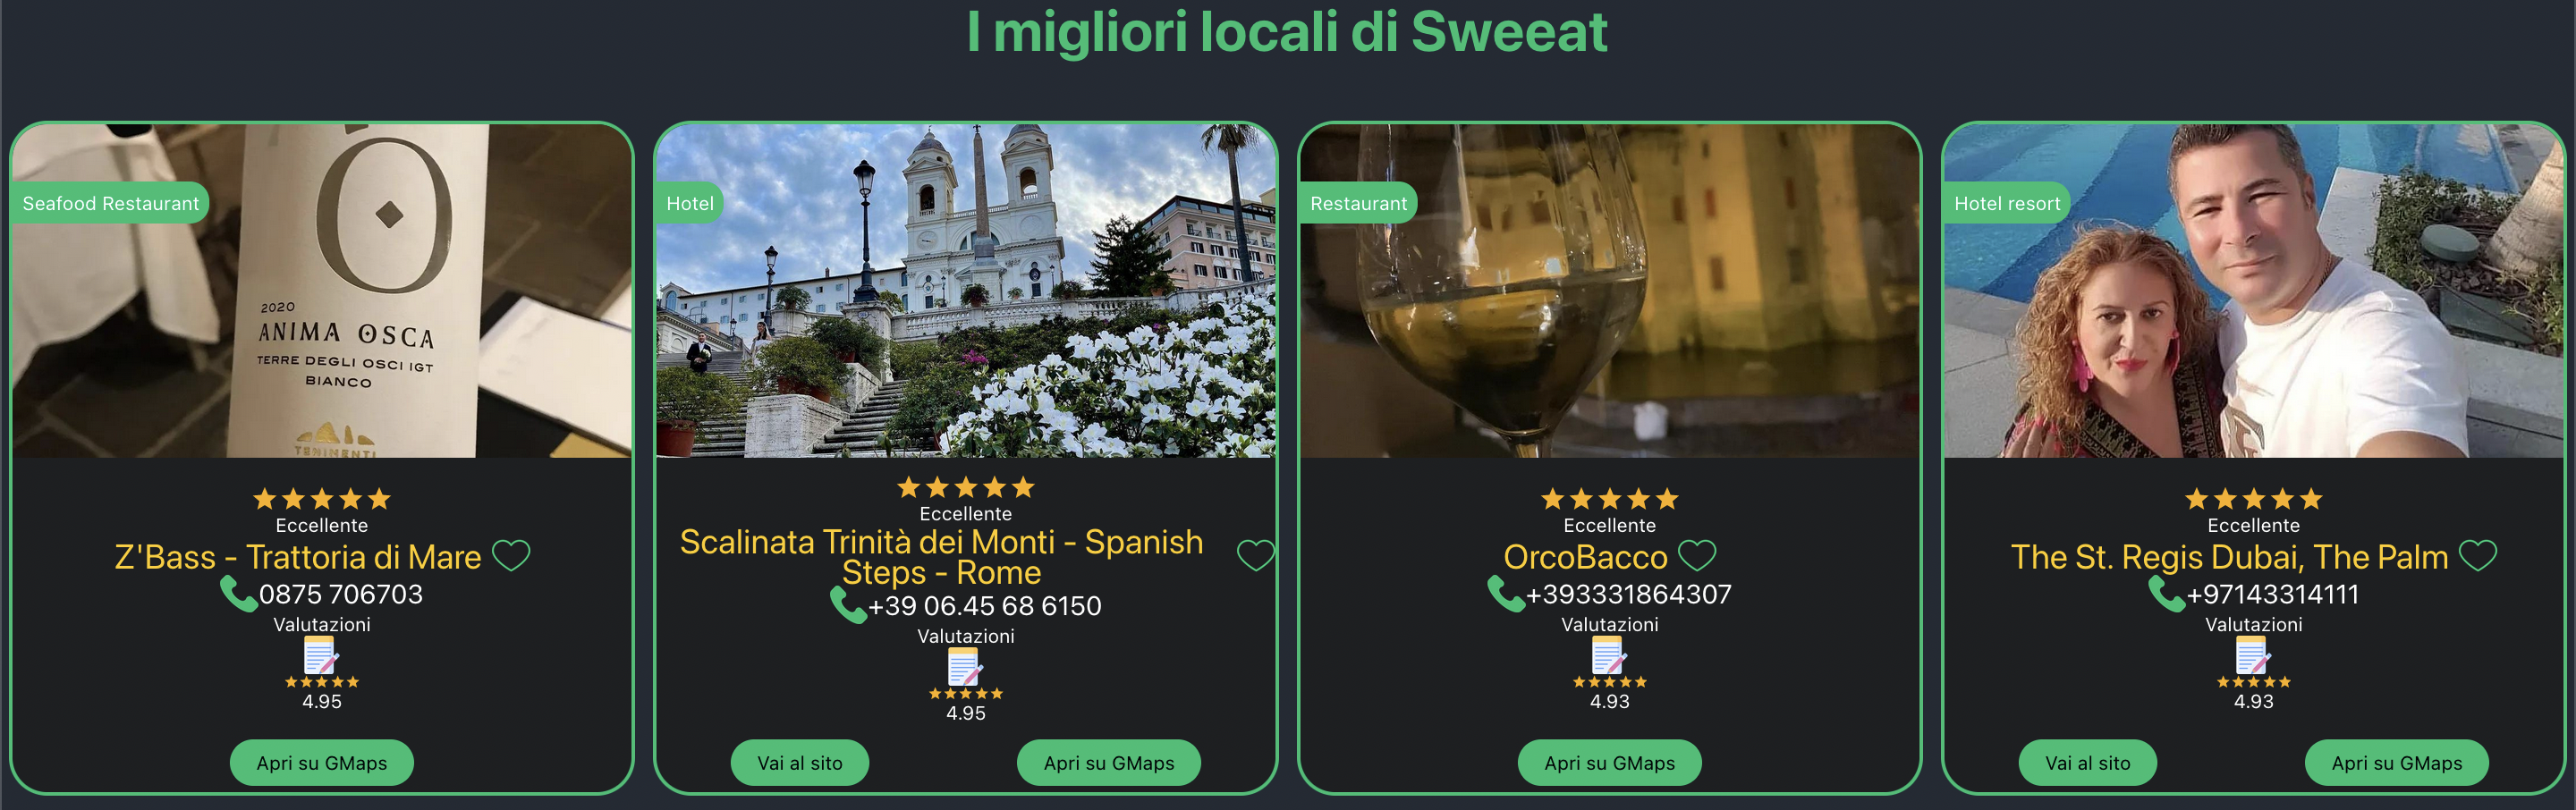
\includegraphics[scale=0.3]{./images/Homepage/MiglioriLocali.png} 
\caption{Inserimento dati ed avvio ricerca in Homepage}
\end{figure}

Per ciascun locale è possibile visualizzare le seguenti informazioni:

\begin{itemize}
\item Nome locale,
\item Valutazione complessiva,
\item Numero di telefono (opzionale),
\item Categoria,
\item Immagine di copertina,
\item Valutazione(*) per:
\begin{itemize}
\item Foto,
\item Testo,
\item Emoticons,
\end{itemize}
\item Link al sito web,
\item Link alla posizione del locale su Google Maps,
\item Possibilità di aggiungere o rimuovere il locale alla lista dei preferiti (funzionalità non ancora implementata).
\end{itemize}

\begin{figure}[H]
\centering
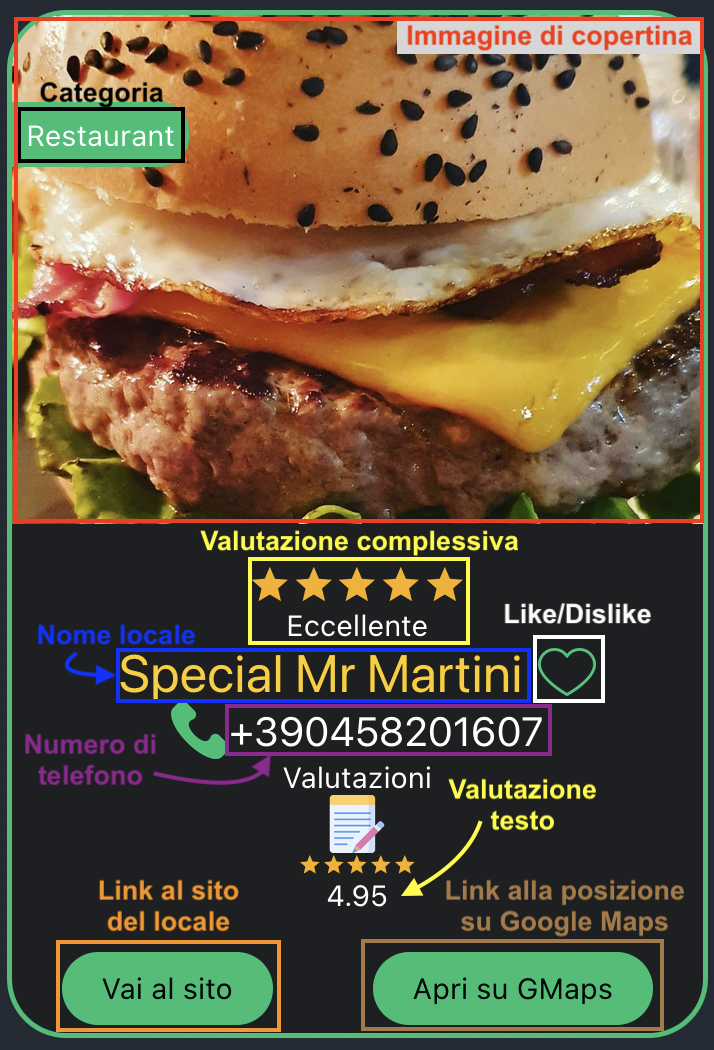
\includegraphics[scale=0.4]{./images/Homepage/Card.png} 
\caption{Card Locale in Homepage}
\end{figure}

(*) Per conoscere il significato delle valutazioni, consulta il paragrafo \S{9.2.1}. \\

La classifica dei migliori locali ha diverse pagine e per scorrerle è necessario cliccare su uno dei numeri presenti nella parte inferiore della pagina.

\begin{figure}[H]
\centering
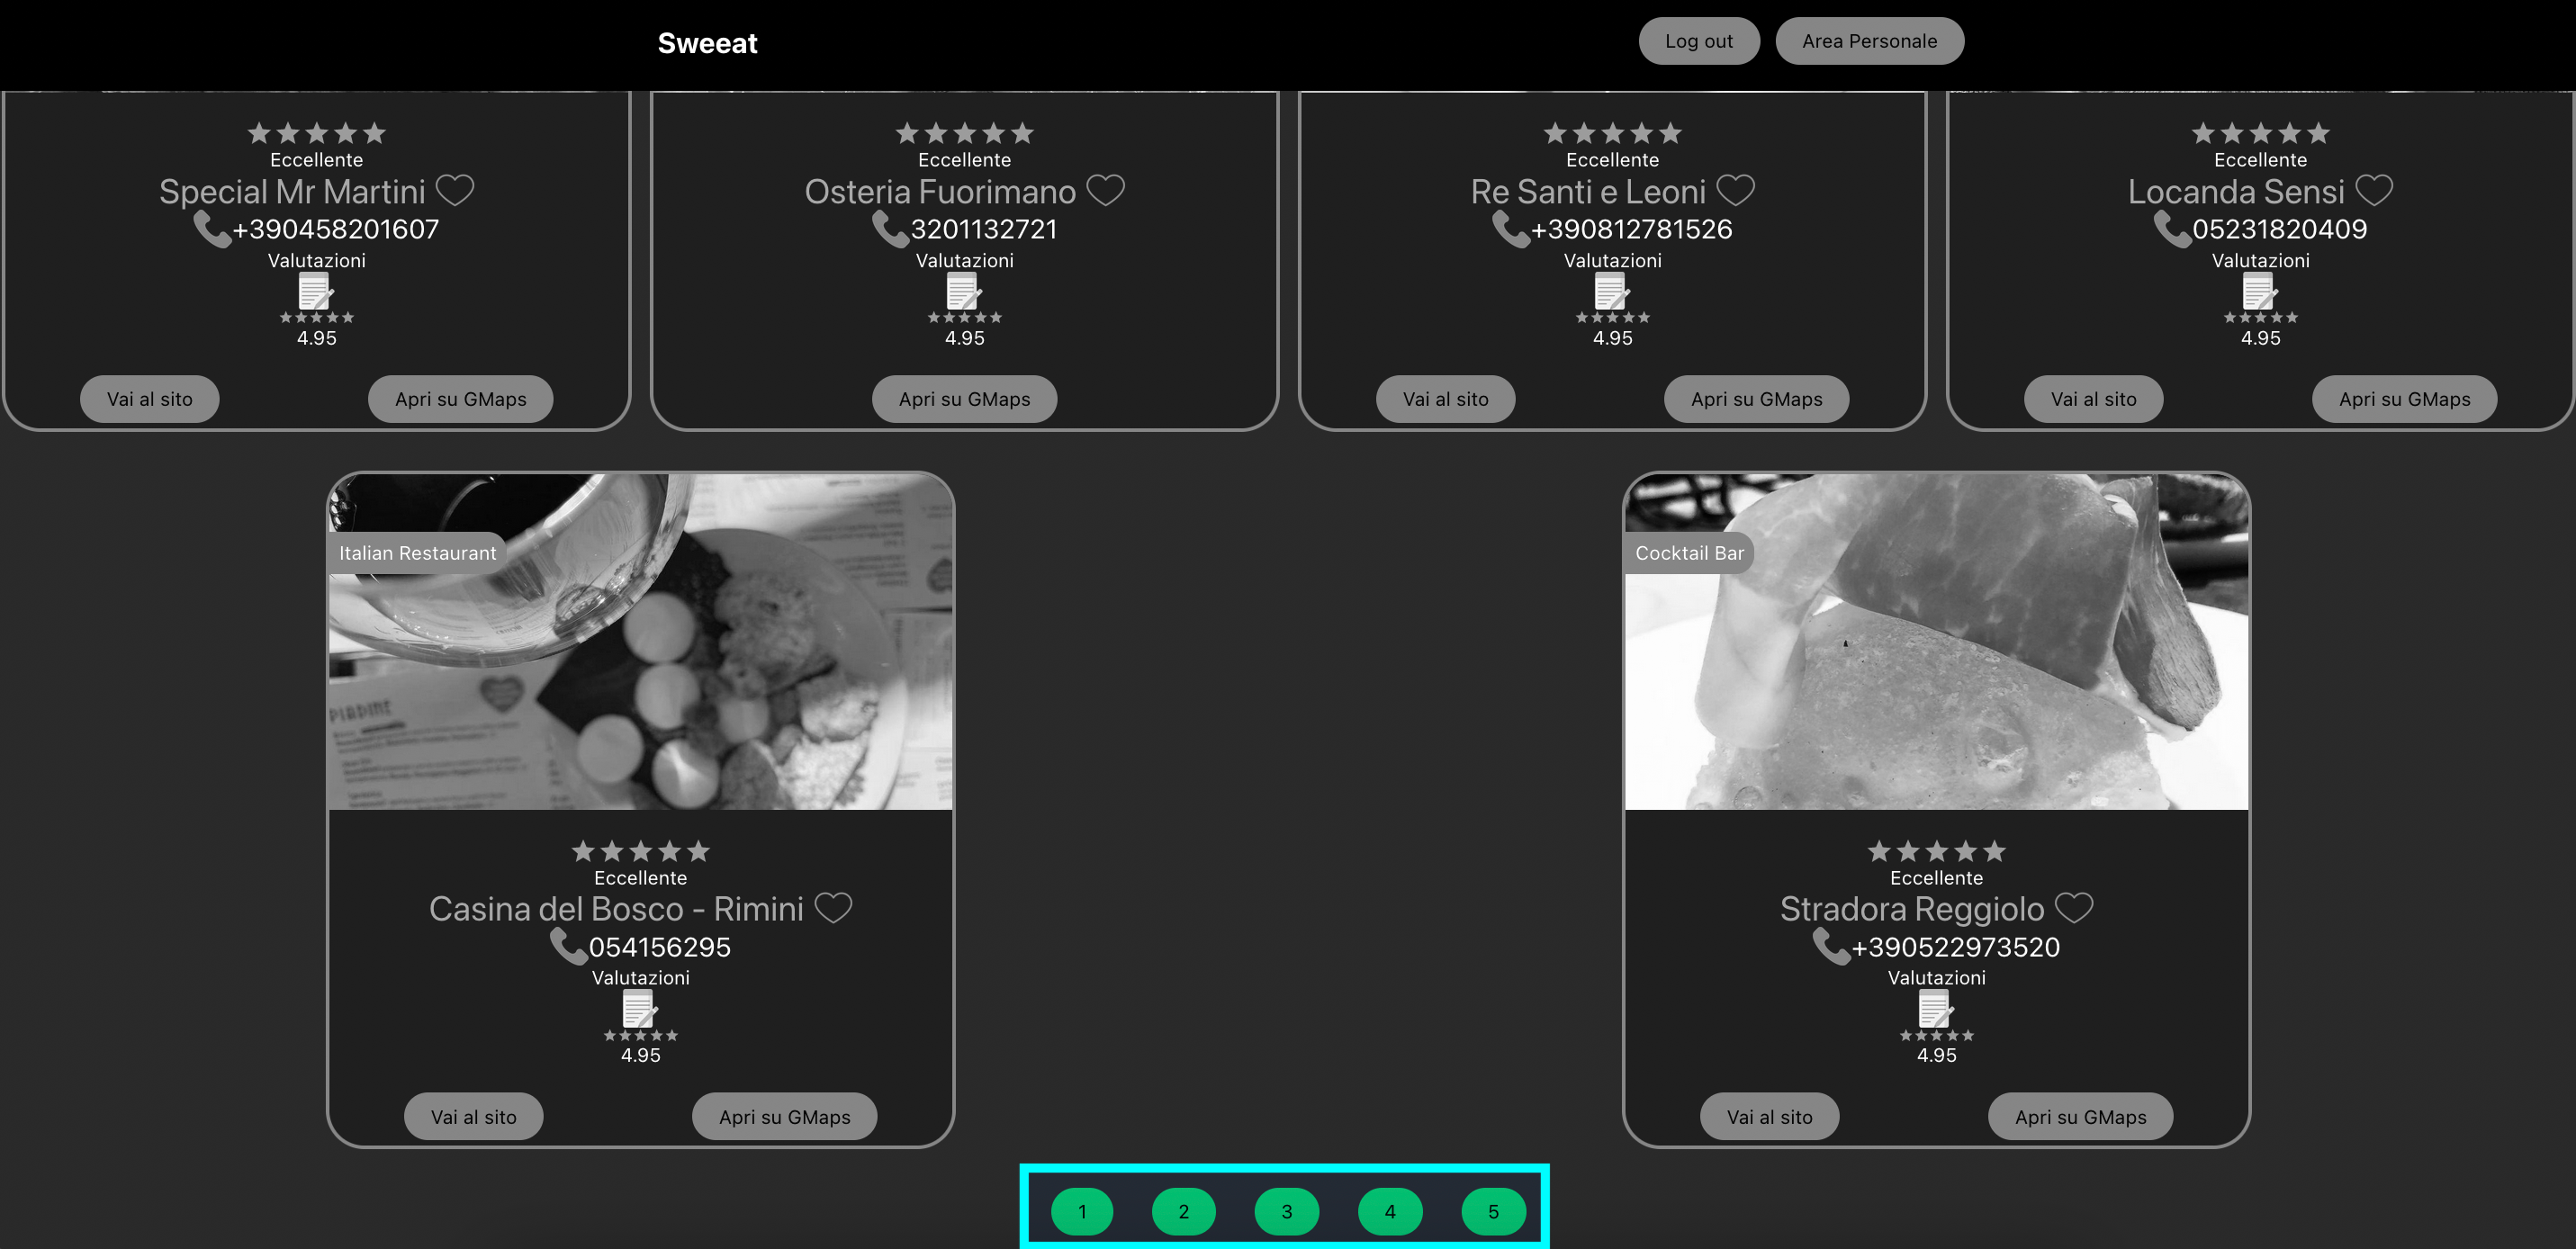
\includegraphics[scale=0.15]{./images/Homepage/Pagine.png} 
\caption{Visualizza altri migliori locali in Homepage}
\end{figure}

Inoltre, cliccando sul nome del locale all’utente verrà mostrata la \textbf{Pagina di dettaglio locale} (\S{10}) la quale, oltre al nome del locale e le informazioni di base appena descritte, conterrà i contenuti multimediali relativi a quel locale pubblicati su Instagram ed utilizzati per realizzare la WebApp.

		
		\section{Visualizza i Risultati}
		% Pagina dei risultati

Una volta inserito il nome del locale da cercare nella barra di ricerca presente in Homepage (\S{8.1}) e cliccato sul bottone “Cerca”, all’utente verranno mostrati i risultati sotto forma di lista in una nuova pagina web, la quale conterrà il locale cercato (o i locali cercati, se ce ne sono più di uno con lo stesso nome) oppure, nel caso il locale non sia presente nel sistema, dei locali alternativi.

\begin{figure}[H]
\centering
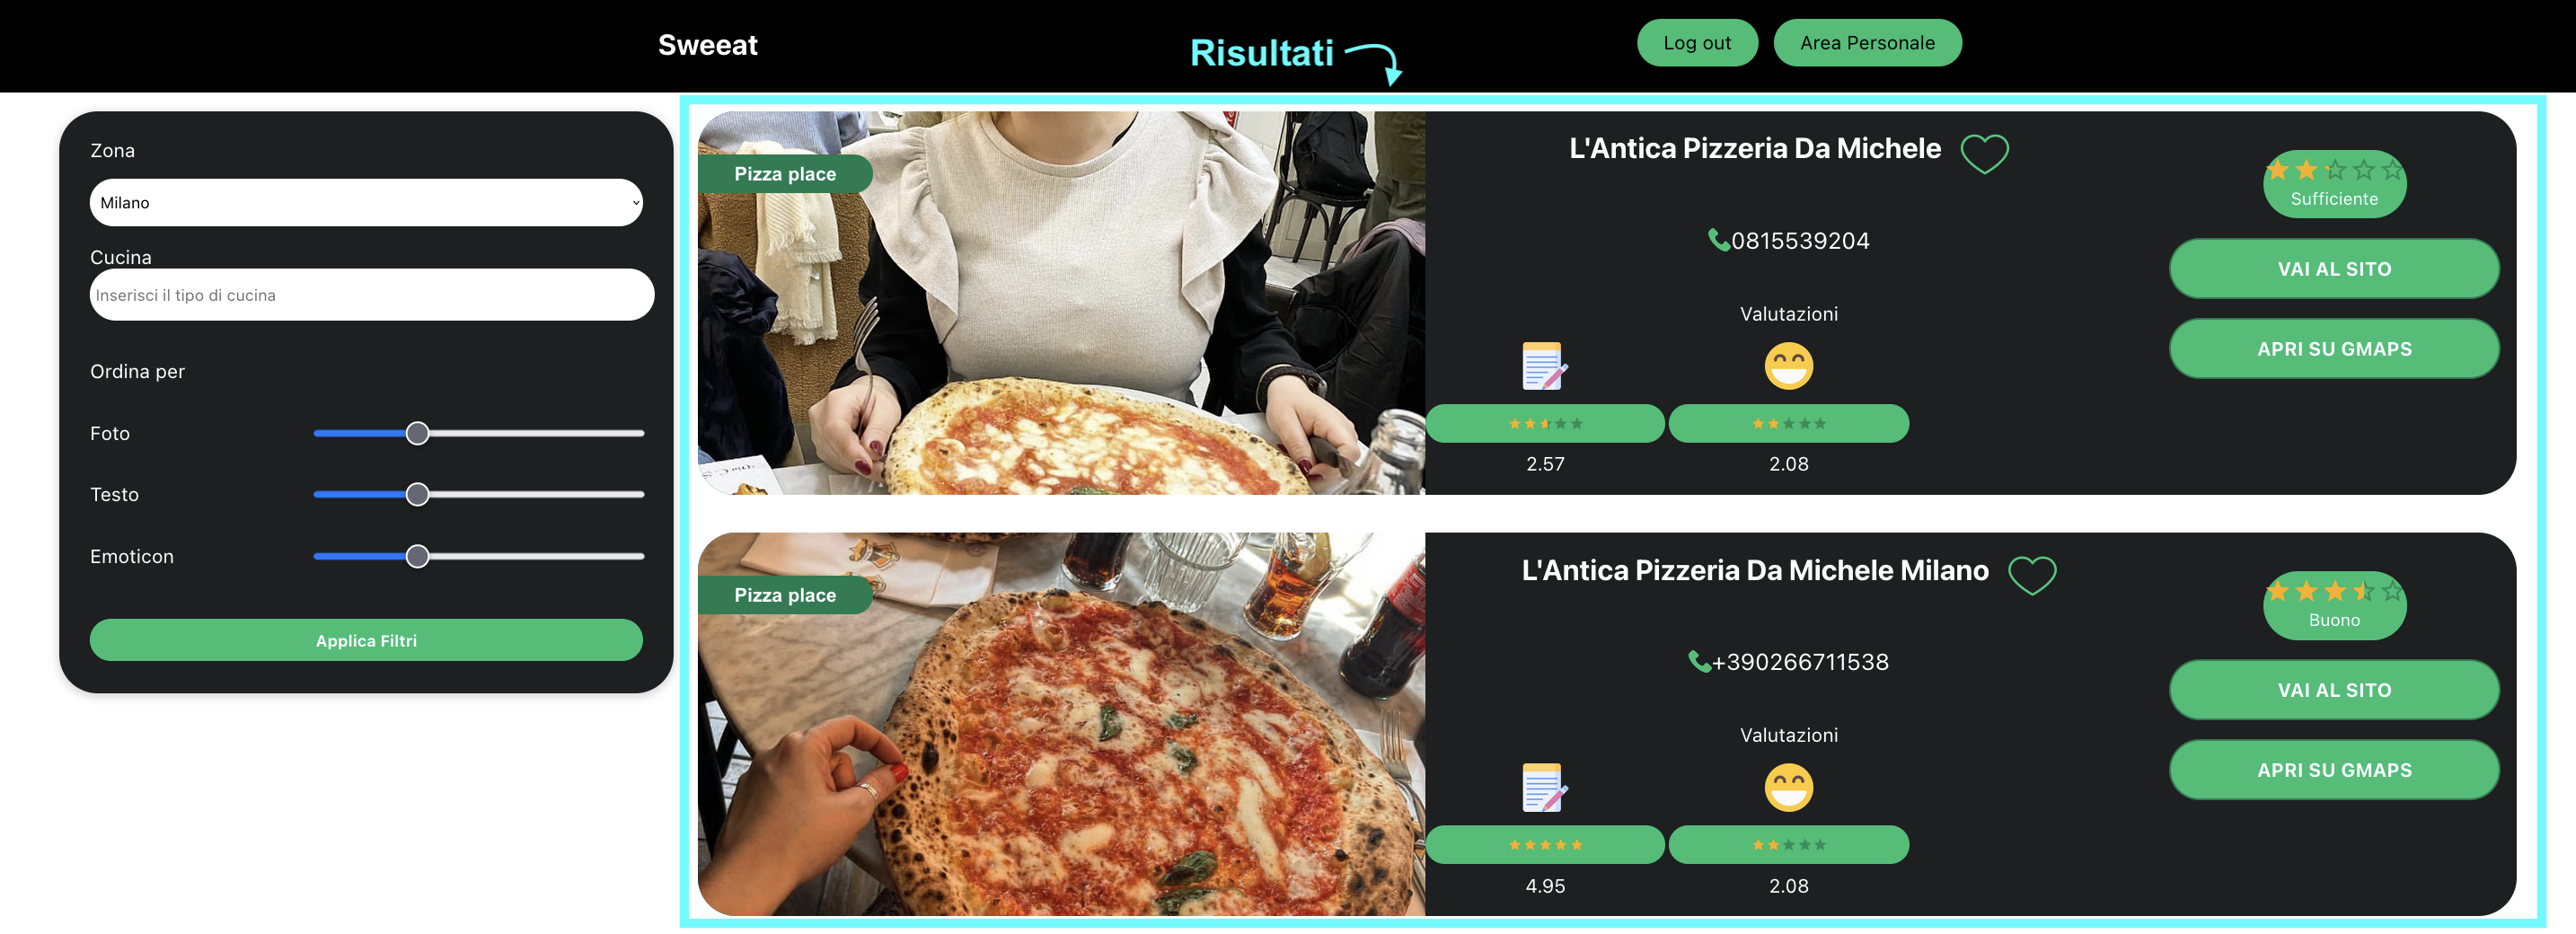
\includegraphics[scale=0.3]{./images/Ricerca/Ricerca.png} 
\caption{Pagina dei risultatati}
\end{figure}

I risultati mostreranno uno o più locali e, per ciascuno di essi, verranno mostrate le seguenti informazioni:

\begin{itemize}
\item Nome locale,
\item Valutazione complessiva,
\item Numero di telefono (opzionale),
\item Categoria,
\item Immagine di copertina del locale,
\item Valutazione per:
\begin{itemize}
\item Foto,
\item Testo,
\item Emoticon,
\end{itemize}
\item Link al sito web,
\item Link alla posizione del locale su Google Maps,
\item Possibilità di aggiungere o rimuovere il locale alla lista dei preferiti (funzionalità non ancora implementata).
\end{itemize}

\begin{figure}[H]
\centering
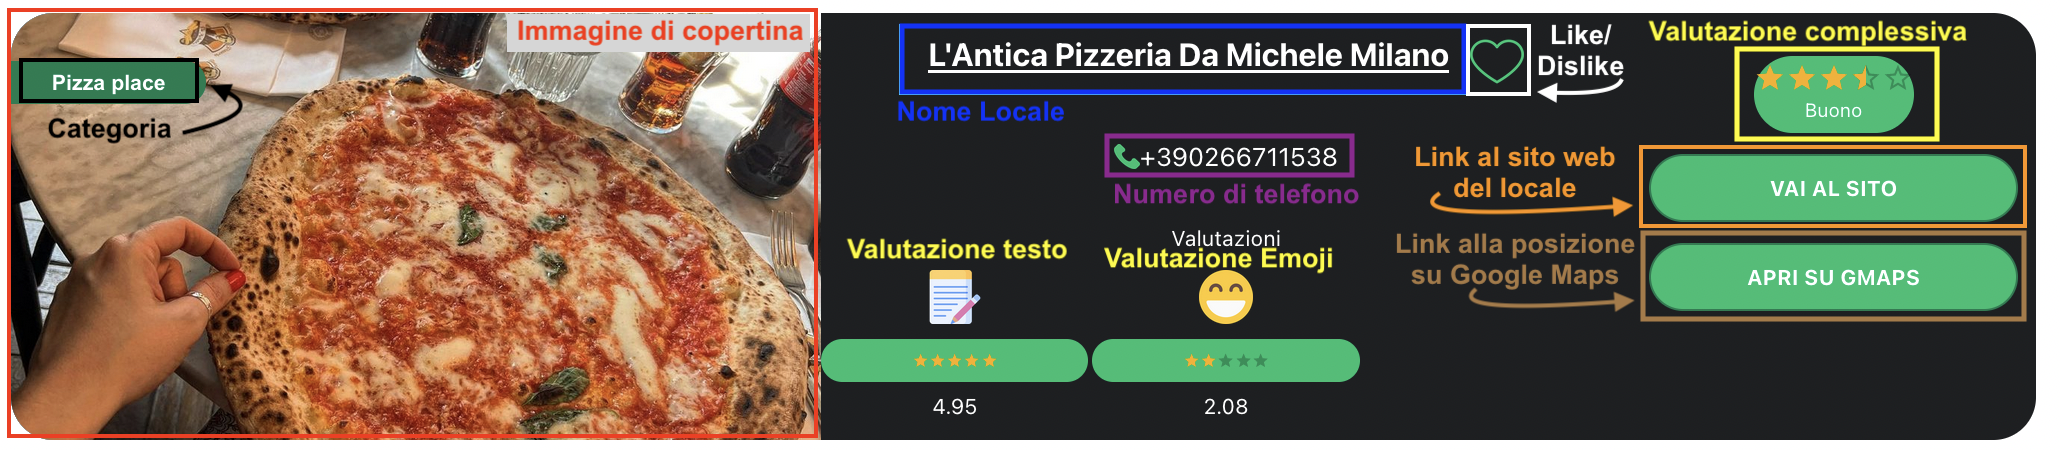
\includegraphics[scale=0.4]{./images/Ricerca/Card.png} 
\caption{Card locale nella pagina dei risultati}
\end{figure}

Inoltre, cliccando sul nome del locale all’utente verrà mostrata la pagina di dettaglio locale (\S{10}) la quale, oltre al nome del locale e le informazioni di base appena descritte, conterrà i contenuti multimediali relativi a quel locale pubblicati su Instagram ed utilizzati per realizzare la WebApp.

Nel caso la ricerca non vada a buon fine e non vengano trovati dei risultati, l’utente visualizzerà il seguente messaggio:

\begin{figure}[H]
\centering
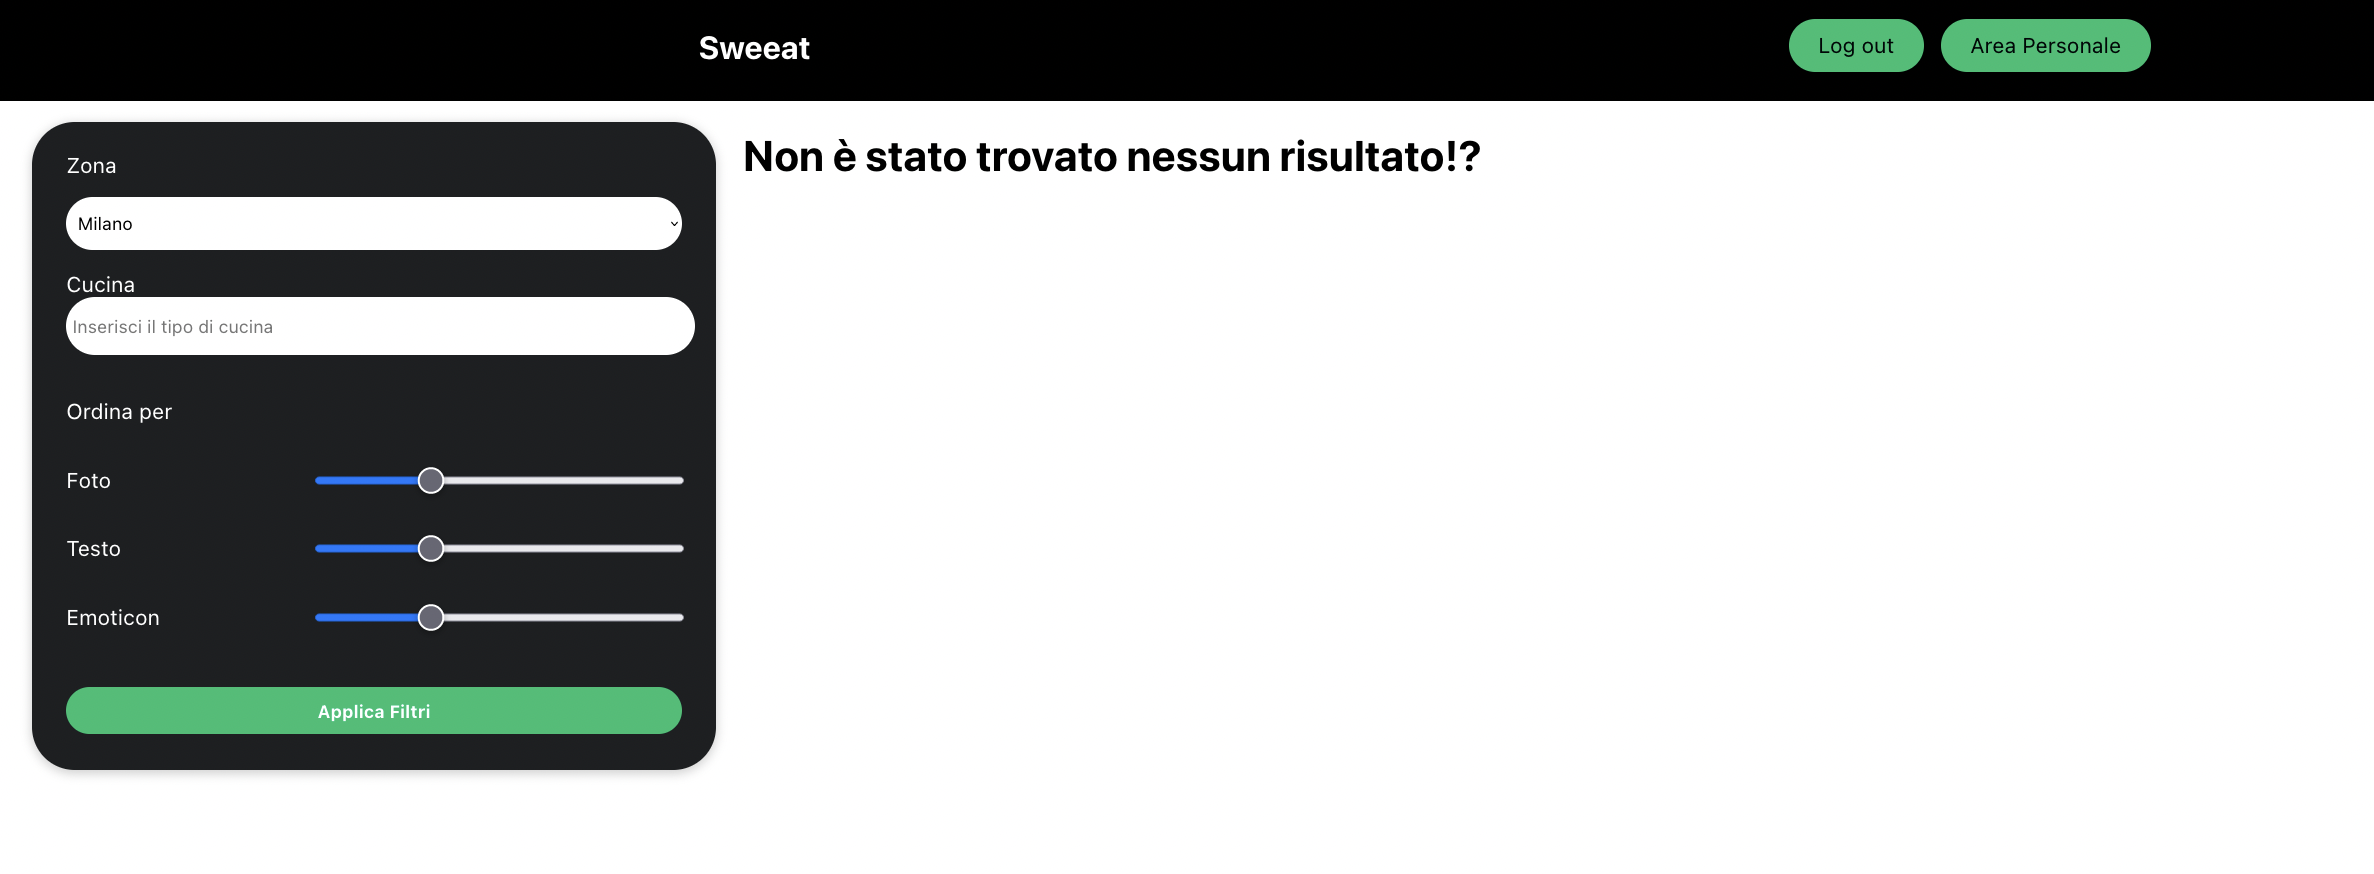
\includegraphics[scale=0.3]{./images/Ricerca/ZeroRisultati.png} 
\caption{Nessun risultato trovato per la ricerca}
\end{figure}

\subsection{Inserimento di un locale nella lista dei preferiti dalla classifica (solo per utenti registrati)}

Se l’utente ha effettuato il login (\S{5}) (tramite indirizzo e-mail e password), oltre alle informazioni di base del locale, accanto al nome del locale troverà l’icona a forma di cuore, che potrà essere:

\begin{itemize}
\item Rossa, se il locale è stato inserito nella lista dei preferiti (\S{7.4}),
\item Vuoto e con il bordo verde, nel caso in cui il locale non sia presente nella lista dei preferiti.
\end{itemize}

\begin{figure}[H]
\centering

\includegraphics[scale=0.6]{./images/Ricerca/Cuore.png} 
\caption{Inserimento/Rimozione locale nella lista dei preferiti}
\end{figure}

Un utente può inserire il locale nella propria lista dei preferiti semplicemente cliccando sopra al cuore vuoto con la cornice verde, mentre può rimuoverlo cliccando sul cuore rosso.

Questa funzionalità è disponibile sia da dispositivo desktop che da mobile; tuttavia, non è ancora stata implementata.

\subsection{Valutazioni}

Per ciascun locale presente nella piattaforma vengono mostrate le valutazioni di:

\begin{itemize}
\item Foto,
\item Testo,
\item Emoticon,
\item Valutazione complessiva.
\end{itemize}

Di base, la valutazione complessiva mostrata è data dalla somma delle valutazioni dei contenuti di foto, testo ed emoticon (in egual misura) di ciascun locale.

La valutazione complessiva delle foto è data dalle immagini pubblicate sui post Instagram e relative al locale in questione, analogamente viene svolto per testo (ossia, i testi dei post delle immagini) ed emoticon (ossia, il grado di soddisfazione del locale da parte dei volti che compaiono nelle immagini pubblicate sui post instagram).

\subsubsection{Il significato delle valutazioni}

Le valutazioni che esprimono la bontà del locale vengono espresse sotto forma di valore numerico ed il loro valore sarà compreso tra 1 e 5. Possiamo sintetizzare il significato del valore numerico come segue:

\begin{itemize}
\item \textbf{1}: pessimo-scarso,
\item \textbf{2}: scarso-sufficiente,
\item \textbf{3}: discreto-punteggio medio,
\item \textbf{4}: buono-ottimo,
\item \textbf{5}: ottimo-eccellente.
\end{itemize}

In sostanza, più il numero della valutazione si avvicina al “5”, migliore sarà la sua reputazione.

\subsection{Filtrare i risultati}

Al fine di ottenere una lista di risultati personalizzati in base all’interesse dell’utente, è possibile applicare dei filtri sulla classifica.

Attualmente, Sweeat offre i seguenti filtri:

\begin{itemize}
\item Per zona geografica (funzionalità non ancora implementata),
\item Per tipo di cucina (funzionalità non ancora implementata).
\end{itemize}

L’utente può impostare la zona geografica d’interesse spostandosi sulla mappa di Google Maps.

Oppure digitando il nome del tipo di cucina d’interesse nella casella di testo.

\begin{figure}[H]
\centering
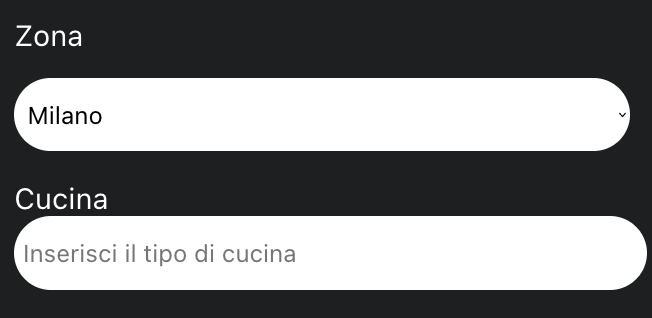
\includegraphics[scale=0.4]{./images/Ricerca/Filtri.png} 
\caption{Filtrare i risultatati - versione desktop}
\end{figure}

\begin{figure}[H]
\centering
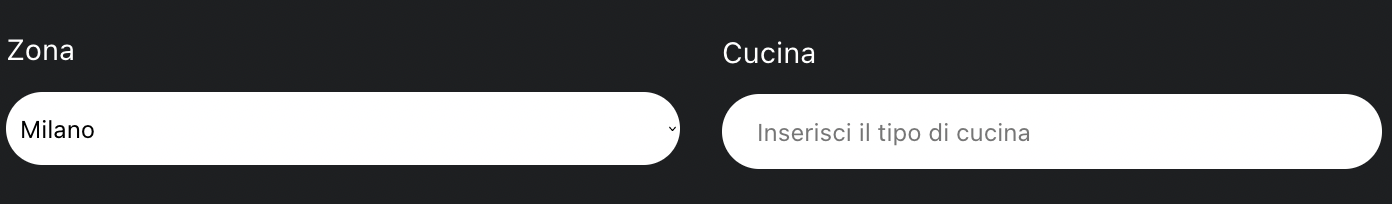
\includegraphics[scale=0.4]{./images/Ricerca/FiltriMobile.png} 
\caption{Filtrare i risultatati - versione mobile}
\end{figure}

\subsection{Ordinare i risultati}

L’utente può anche modificare l’ordinamento dei risultati impostando il peso su ciascuno dei seguenti contenuti:

\begin{itemize}
\item Foto (funzionalità non ancora implementata),
\item Testo (funzionalità non ancora implementata),
\item Emoticon (funzionalità non ancora implementata).
\end{itemize}

L’utente può impostare il peso di ciascuno di questi contenuti tramite:

\begin{itemize}
\item Lo slider, nella versione Desktop (funzionalità non ancora implementata), 
\item Impostando un valore dal menù a tendina, nella versione mobile (funzionalità non ancora implementata).
\end{itemize}

\begin{figure}[H]
\centering
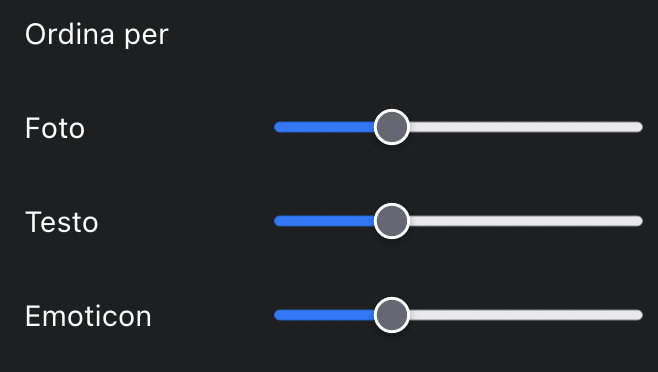
\includegraphics[scale=0.4]{./images/Ricerca/Ordina.png} 
\caption{Ordinare i risultatati - versione desktop}
\end{figure}

\begin{figure}[H]
\centering
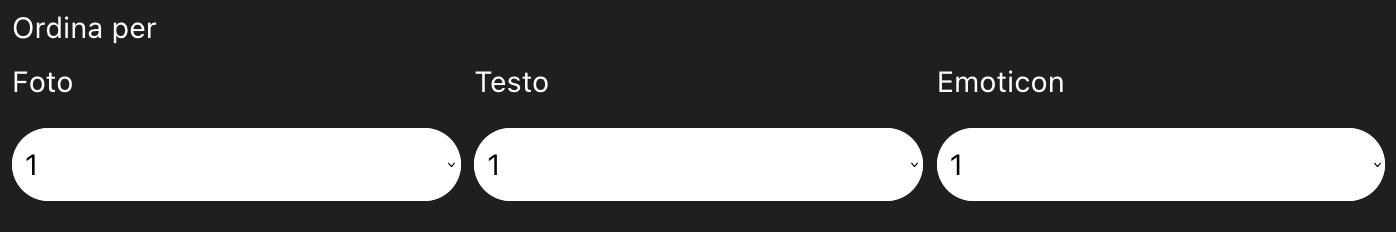
\includegraphics[scale=0.4]{./images/Ricerca/OrdinaMobile.png} 
\caption{Ordinare i risultatati - versione mobile}
\end{figure}

I valori del menù a tendina sono i seguenti:

\begin{itemize}
\item \textbf{1}: pessimo-scarso,
\item \textbf{2}: scarso-sufficiente,
\item \textbf{3}: discreto-punteggio medio,
\item \textbf{4}: buono-ottimo,
\item \textbf{5}: ottimo-eccellente.
\end{itemize}

\subsection{Applicare i filtri ed ordinare i risultati}

Una volta impostati i filtri ed il peso di ogni contenuto, affinché l’utente possa ottenere una lista con dei risultati personalizzati in base alle sue scelte, dovrà cliccare sul bottone “\textbf{Applica Filtri}”.

\begin{figure}[H]
\centering
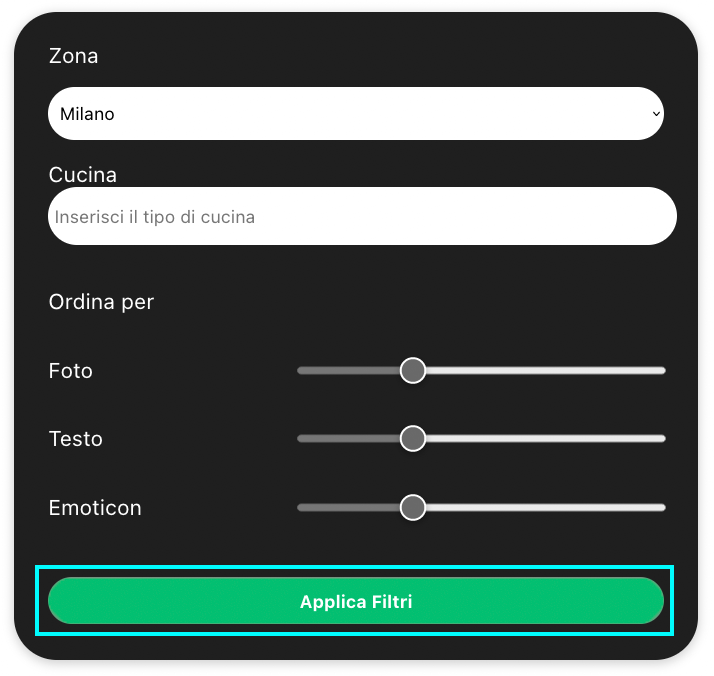
\includegraphics[scale=0.3]{./images/Ricerca/ApplicaFiltri.png} 
\caption{Come applicare i filtri ed ordinare i risultati}
\end{figure}
		
		
		\section{Pagina di dettaglio locale}
		% Pagina di dettaglio locale

È possibile visualizzare le informazioni di un locale cliccando sul nome del locale di interesse dalla classifica.

\begin{figure}[H]
\centering
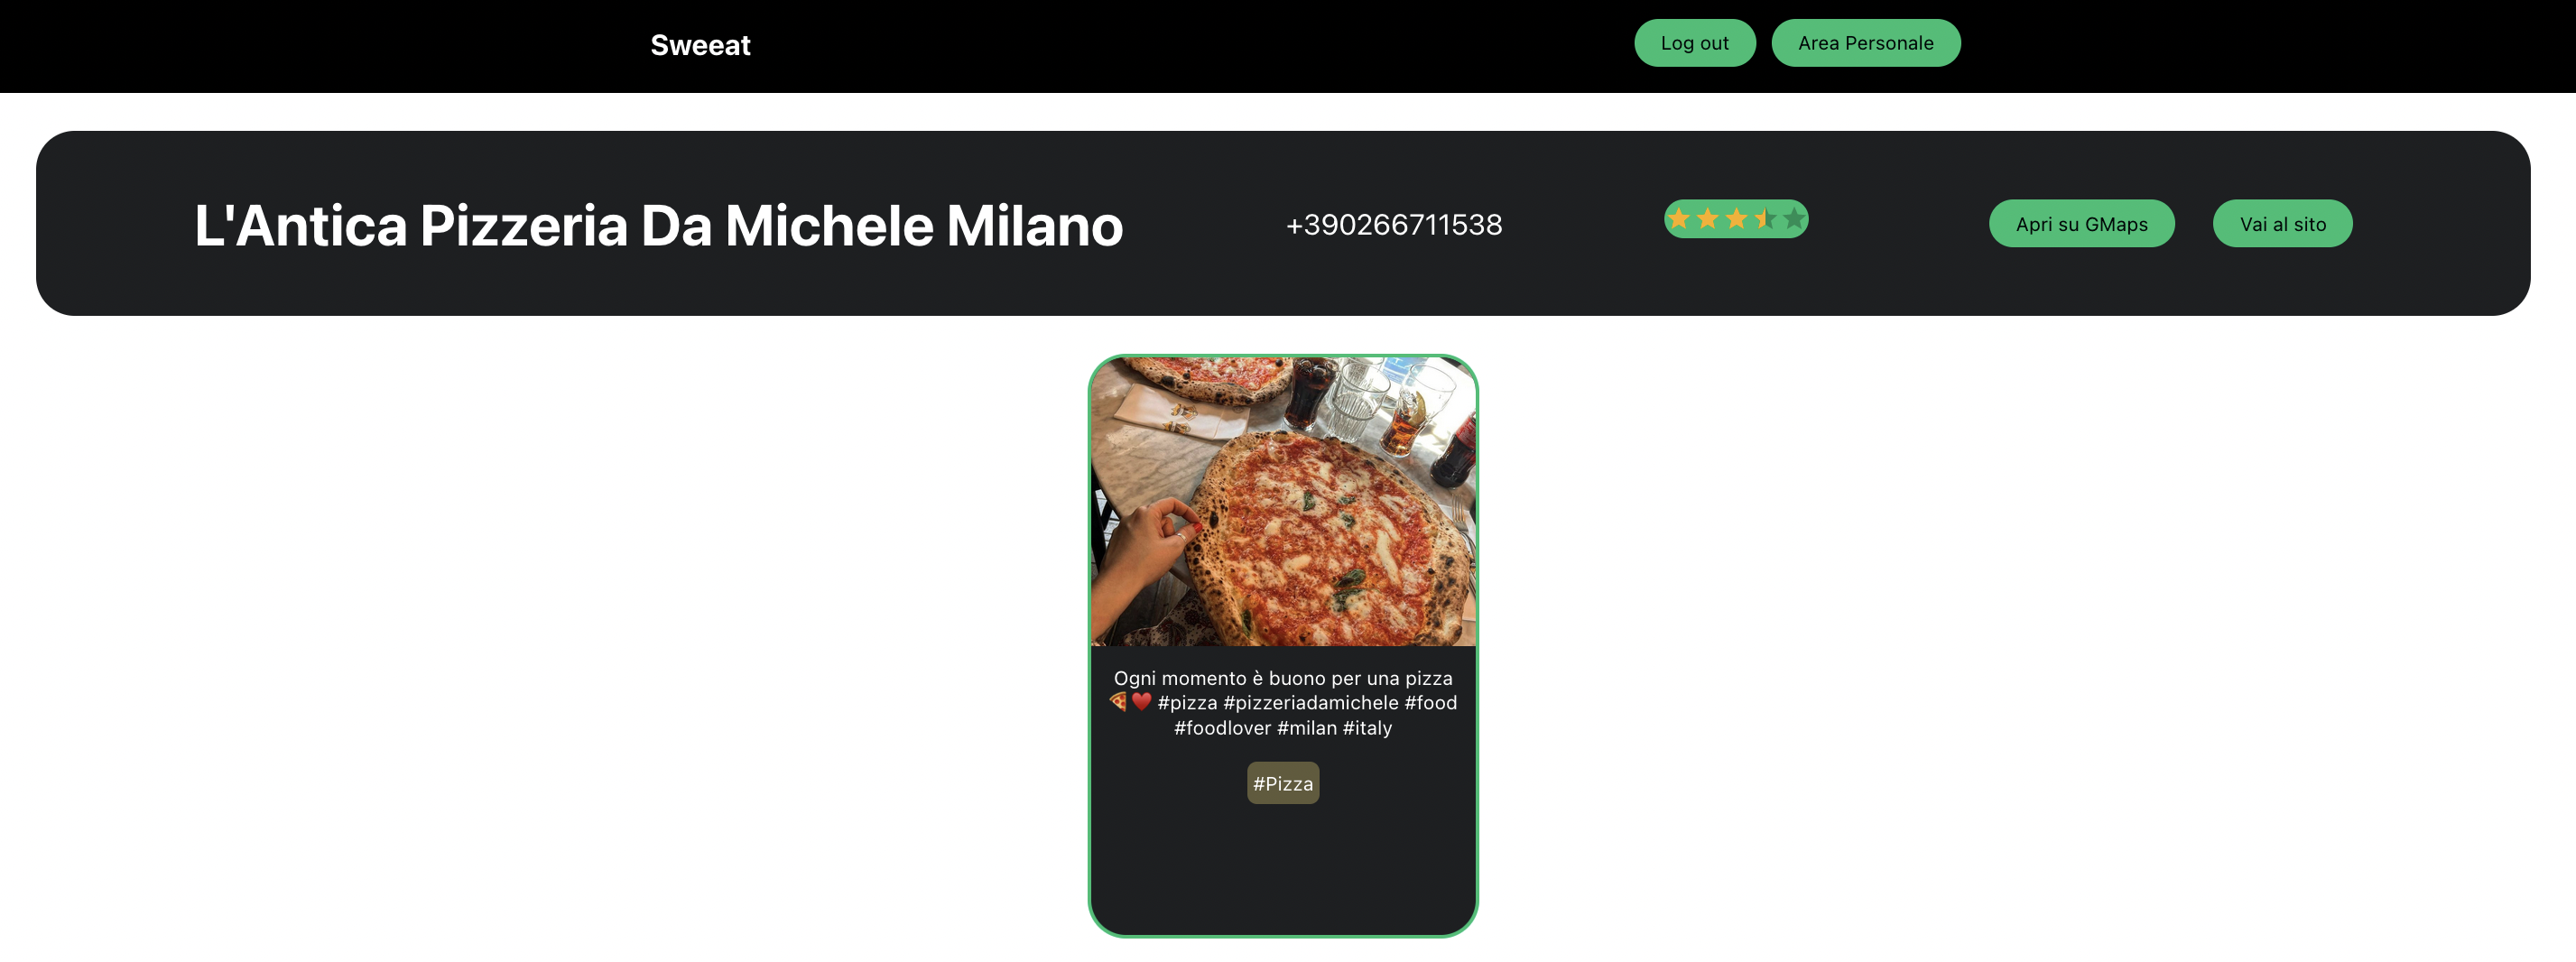
\includegraphics[scale=0.3]{./images/DettagliLocale/DettagliLocale.png} 
\caption{Pagina di dettaglio locale}
\end{figure}

Una volta cliccato sul nome del locale, all’utente verrà mostrata una nuova pagina che conterrà i seguenti dettagli:

\begin{itemize}
\item Nome locale,
\item Numero di telefono del locale,
\item Link al sito web del sito (nel caso ci sia),
\item Link alla posizizione di GMaps del locale,
\item Valutazioni:
\begin{itemize}
\item Complessiva,
\item Foto, 
\item Testo,
\item Emoji.
\end{itemize}
\end{itemize}

Inoltre, sono presenti anche uno o più post pubblicati su Instagram e relativi al locale di cui si sta visualizzando la pagina di dettaglio.
Per ciascun post vengono mostrati:

\begin{itemize}
\item Immagini del post,
\item Testo del post,
\item Tag relativi alle immagini del post.
\end{itemize}

Attualmente, viene mostrata solo la prima immagine del post.

\begin{figure}[H]
\centering
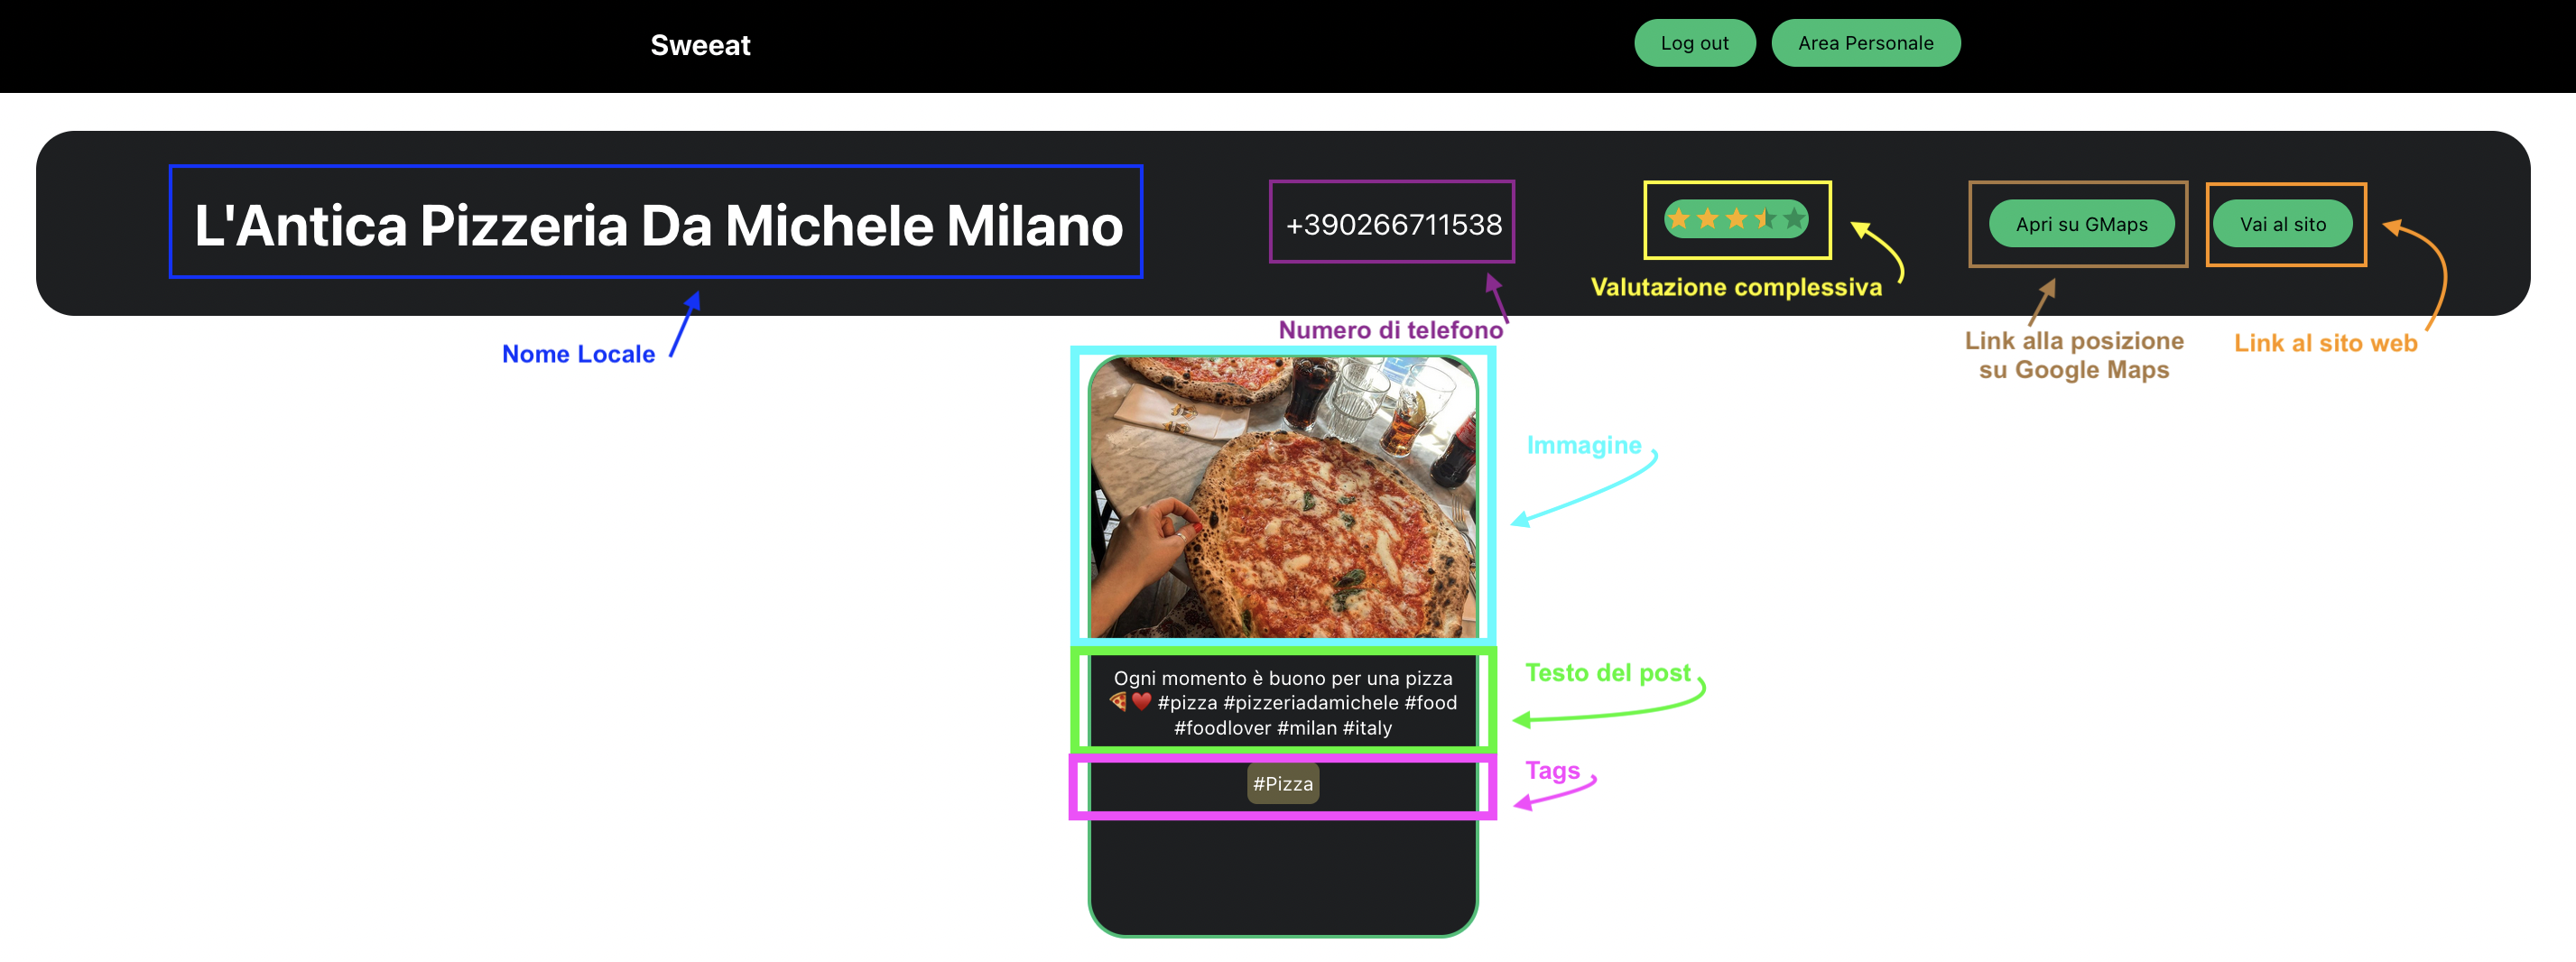
\includegraphics[scale=0.3]{./images/DettagliLocale/DettagliLocale2.png} 
\caption{Informazioni visualizzate pagina di dettaglio locale}
\end{figure}
		
\end{document}